\newcommand{\di}{\ensuremath{\mathrm{\,d}}}
\newcommand{\Mul}{\ensuremath{\mathsf M}}
\newcommand{\A}{\ensuremath{\mathbb A}}
\newcommand{\R}{\ensuremath{\mathsf R}}
\newcommand{\IZ}{\ensuremath{{I \backslash \{0\}}}}
\newcommand{\me}{\mathrm{e}}

\newcommand\DOI[1]{doi: \href{http://doi.org/#1}{\texttt{#1}}}
\newcommand\ARXIV[1]{arxiv: \href{https://arxiv.org/abs/#1}{\texttt{#1}}}

\allowdisplaybreaks

\makeatletter
\newenvironment{breakablealgorithm}
  {% \begin{breakablealgorithm}
   \begin{center}
     \refstepcounter{algorithm}% New algorithm
     \hrule height.8pt depth0pt \kern2pt% \@fs@pre for \@fs@ruled
     \renewcommand{\caption}[2][\relax]{% Make a new \caption
       {\raggedright\textbf{\ALG@name~\thealgorithm} \sc##2\par}%
       \ifx\relax##1\relax % #1 is \relax
         \addcontentsline{loa}{algorithm}{\protect\numberline{\thealgorithm}##2}%
       \else % #1 is not \relax
         \addcontentsline{loa}{algorithm}{\protect\numberline{\thealgorithm}##1}%
       \fi
       \kern2pt\hrule\kern2pt
     }
  }{% \end{breakablealgorithm}
     \kern2pt\hrule\relax% \@fs@post for \@fs@ruled
   \end{center}
  }
\makeatother

\begin{abstract}
生成函数近年来在信息学竞赛的组合计数问题中扮演着越加重要的角色。其用途在问题处理时的公式推导,以及代码实现中的学问均已逐渐普及。本文旨在给出一套生成函数在信息学竞赛实战中处理问题的方法框架,同时梳理一些其中的重要算法。
\end{abstract}

\ifcont

\tableofcontents

\newpage

\fi

\section{概述}

当我们得到一个组合计数问题相关的生成函数解后,其代数形式到答案计算的算法的转化过程仍有若干壁垒。究其原因,我们在进行计算时常常受到以下几个复杂对象的制约。

\subsection{复合}

相对于卷积,我们在形式幂级数问题上没有非常高效的处理一般复合问题的方法。多项式模复合问题在 OI 中已经被引入的复杂度最优的算法为 $\Theta((n\log n)^{3/2})$,且该算法具有较大的常数,在实战中往往 $\Theta(n^2)$ 次运算的一种“分块 FFT”算法具有更好的表现。值得一提的是,该问题在理论界已有 $O(n^{1+o(1)})$ 的算法(见 \cite{polyfact}),但尚不清楚在实现上是否优越。

\subsection{生成函数方程}

当组合对象的描述中进行自指时,生成函数方程便自然产生。在方程中种种运算的复合会使得计算更为困难。例如组合对象的笛卡尔积导出生成函数的乘积 $A(x)\times B(x)$,结构的复合导出生成函数的复合 $A(B(x))$,EGF 中对位置的固定导出生成函数的微分 $A'(x)$,P\'olya 计数定理导出下标变换 $A(x^k)$ 等。

\subsection{远处系数求值}

远处系数求值意谓在提取第 $n$ 次项系数时,往往 $\Omega(n)$ 的计算量都是不被允许的。而能在 $o(n)$ 时间内完成计算的问题要求确实比较苛刻,但目前仍有一些可探讨的空间。目前较为成熟的两类远处系数求值是\emph{线性递推数列}和\emph{整式递推数列}。

\begin{theorem}给定数列 $a_n$ 的 $0\sim k-1$ 项和定义在其上的线性递推式 $b_1,\dots, b_k$,满足
$$ a_n = \sum_{j=1}^k a_{n-j} b_j $$

存在算法在 $\Theta(k\log k\log n)$ 时间内计算 $a_n$。
\end{theorem}

现在较为普及的线性递推算法由 Fiduccia 于 1985 年提出,并不具有较好的常数。后文将介绍一种算法上更为简单,且具有较好常数的线性递推算法。

\begin{theorem}给定数列 $a_n$ 的 $0\sim m-1$ 项和定义在其上的整式递推式 $P_0,\dots,P_m$,其中 $P$ 皆为不超过 $d$ 次多项式,满足
$$ a_n = -\frac1{P_0(n)}\sum_{j=1}^m a_{n-j}P_j(n) $$

存在算法在 $\Theta \left(\sqrt{nd}\left(m^3+m^2\log(nd)\right)\right)$ 时间内计算 $a_n$。
\end{theorem}

\subsection{线性变换}

在对序列进行的线性变换中,有一类变换是极常见的,其变换可以用多项式的表示方法描述。围绕多项式的单项式系数表示和下降幂系数表示,下列等式
$$
f(x) = \sum_{n\le N} a_n x^n = \sum_{n\le N} b_n x(x-1)\dots (x-n+1)
$$
中,序列 $a$ 与 $b$ 的相互转化目前有 $\Theta(n\log ^2n)$ 的复杂度这一壁垒。但在各自的表示之下,二者在进行其他运算时却常常具有不同的优势,各自在一类问题上具有 $\Theta(n\log n)$ 或者 $\Theta(n)$ 的复杂度。

此外,在处理线性变换时,转置原理可以帮助我们简化问题。

\ifcont
\paragraph{${\textbf{转} \atop \textbf{置}}$原理}
\else
\paragraph{转置原理}
\fi
\cite{tellegen} 指出,在考虑一类可表示为对输入向量 $\mathbf x$ 进行矩阵乘法 $\mathbf {Mx}$ 的计算时,可考虑先对 $\mathbf M^{\mathsf T}\mathbf y$ 的计算设计算法,然后将算法的各步骤转置改写。

\section{算法的评定}

\subsection{系数}

在信息学竞赛的组合计数问题中,由于问题常常要求输出对某个数取模的结果,而这一计算方式往往会影响算法的使用。其对计算复杂程度的影响大致可分为以下四级。

\begin{center}
\begin{tikzcd}[row sep=tiny, column sep=small]
			\mathbb F_{\mathsf{NTT}} \arrow[phantom, r, "\subset" description] & \mathbb F_p \arrow[phantom, r, "\subset" description] & \mathrm{GF}(p^k) \arrow[phantom, r, "\subset" description] & \mathsf{Commutative\ Rings} \\
			\text{NTT 模数域} & \text{素数域} & \text{有限域} & \text{交换环}
\end{tikzcd}
\end{center}

\begin{asparadesc}
\item [NTT 模数域] 设取模的素数 $p$ 满足 $p= m\times 2^k+1$,当 $k$ 较大时,由于 $2^k$ 次单位根的存在,快速数论变换可以在 $\Theta(n\log n)$ 时间内进行长度为 $2$ 的幂,且最长为 $2^k$ 的数论意义下 DFT 结果。由此即可对于 $n\le 2^k$,在 $\Theta(n\log n)$ 的时间内完成两个 $n$ 次多项式的乘法。由于其 DFT 的存在,在这种模数下的算法往往有很大的,根据 DFT 中间结果进行针对性常数优化的空间。

\begin{itemize}
\item \emph{模 $998244353$}:NTT 模数中最为著名的非 $\mathbb F_{998244353}$ 莫属,有 $998244353 = 119\times 2^{23} + 1$。
\end{itemize}

\item [素数域] 在题目中要求答案同余一个素数也较为常见,其中又有大多数情况 $p$ 很大(例如 $10^9+7$),通常是为了保证算法中可以较自由地进行除法。

\item [有限域] 对于一个 $\mathbb F_p$ 上的 $n$ 阶不可约多项式 $f$,$\mathbb F_p[x]/f$ 为一 $p^n$ 阶有限域,记为 $\mathrm{GF}(p^n)$。

\begin{itemize}
\item \emph{Nimber}:Nimber 是一种可以较为高效计算的有限域,其出现时往往为 $\mathrm{GF}(2^{32})$ 或 $\mathrm{GF}(2^{64})$,与计算机的无符号整数 \texttt{uint32} 或 \texttt{uint64} 交相呼应。
\item \emph{二次扩域}:题目中较为常见的是二次扩域,实际上就是对于模 $p$ 下的二次非剩余 $r$,模拟 $a + b\sqrt r$ 的运算。这实际上就等价于 $\mathbb F_p[x]/(x^2-r)$,由 $r$ 是二次非剩余可知 $x^2-r$ 是不可约多项式,故前式是域。
\end{itemize}

\item [交换环] 交换环中不一定有逆,因此并不总能进行除法。

\begin{itemize}
\item \emph{模 $n$ 运算}:$\mathbb Z/n\mathbb Z$ 在 $n$ 是合数时不构成域。
\item \emph{多项式}:若多项式的元素仅构成交换环,或者运算时对一可约多项式取模都会导致运算不构成域,只构成交换环。
\end{itemize}

\item [杂项] 还有部分性质极差的运算,它们并非本文想要讨论的重点,仅简单提及。

\begin{itemize}
\item \emph{矩阵环}:矩阵的乘法是信息学竞赛中最常见的非交换运算。由于其非交换性,在诸如生成函数乘法逆的计算时需要注意运算顺序,而诸如生成函数 $\exp$ 等运算并不具有很好的性质,尚未有复杂度优秀的算法。
\item \emph{最值与最值计数}:最值与最值计数仅构成交换半环,由于目前 max-plus 卷积尚未有 $O(n^{2-\epsilon})$ 的算法,限于其算术性质与本文相离太远,故仅在此提及。
\end{itemize}

\end{asparadesc}

在接下来的表述中,我们默认计算时的系数至少为交换环,记为 $\A$。

\subsection{序列变换}

\subsubsection{卷积}

\begin{definition} [卷积下标系统]
我们称满足以下几条性质的集合 $I$ 以及定义在其上的运算 $\circ$ 构成下文要讨论的\emph{卷积下标系统}:
\begin{itemize}
\item \emph{结合律}:即 $\forall i,j,k\in I$,有 $(i\circ j)\circ k = i\circ(j\circ k)$。
\item \emph{交换律}:对于 $\forall i,j\in I$,有 $i\circ j = j\circ i$。
\item \emph{单位元}:存在元素 $1 \in I$,对于 $\forall i\in I$,有 $1\circ i = i$。
\item \emph{零元}:存在元素 $0\in I$,对于 $\forall i\in I$,有 $0\circ i = 0$。
\item \emph{后效律}:对于 $\forall i \in \IZ$,对任意正整数 $k$ 和 $j_1,\dots,j_k \in I\backslash \{0,1\}$ 有 $i\circ j_1\circ \dots \circ j_k \neq i$。
\end{itemize}
下文中如有歧义时则用 $0_I, 1_I$ 表示 $0,1$。在讨论卷积下标系统时,默认以 $I$ 表示 $(I, \circ)$。在讨论算法时,我们默认 $I$ 是有限的。
\end{definition}

\begin{definition} [生成函数]
对于以卷积下标系统 $I$ 为下标的序列 $\{f_i \in \A\}_{i\in \IZ}$,我们定义其生成函数 $F(X) = \sum_{i\in I} f_i X^i$,我们记 $X$ 为“未定元”,满足:

\begin{itemize}
\item 对 $\forall a\in \A, i\in I$,有 $aX^i = X^i a$。
\item 对 $\forall i,j\in I$,有 $X^i \cdot X^j = X^{i\circ j}$。
\item \emph{消去律}:$X^{0_I} = 0_{\A}$,即 $X^{0_I}$ 作为生成函数对应的序列为 $\{f_i = 0_{\A}\}_{i\in \IZ}$。
\item $X^{1_I} = 1_{\A}$。
\end{itemize}

\end{definition}

容易看出,前文所定义的\emph{零元}刻画了在计算时溢出的部分。

我们记这样的全体生成函数 $F(X)$ 构成的环为 $\mathfrak G[X]$。

我们所选取的生成函数进行乘法时,未定元指标的运算自然地导出了对应系数序列的卷积。

\begin{definition} [卷积]
对于以卷积下标系统 $I$ 为下标,以 $\A$ 为系数的序列,我们定义其卷积 $c = a * b$:
$$
c_k = \sum_{i\circ j = k} a_i b_j
$$
\end{definition}

\begin{definition} [截取]
称 $I'$ 是 $I$ 的一个截取,当且仅当 $\{0,1\}\subseteq I'\subseteq I$ 且 $\forall i\in I\backslash I', \forall j \in I, i\circ j\notin I'\backslash \{0\}$。从而定义运算 $\circ_{I'}$ 为
$$
i\circ_{I'} j = \begin{cases}
i\circ j & i\circ j \in I'\\
0 & \mathrm{else}
\end{cases}
$$
\end{definition}

形象地看,从 $I$ 中截取的 $I'$ 即为删去了 $I$ 中的一部分「边界」,仅保留剩余部分的信息。

\subsubsection{在线算法}

通过前文的铺垫,我们接下来叙述一个静态的算法与其\emph{在线}形式的关联。

\begin{definition} [后效序]
定义 $I$ 上的序关系 $\preceq$:$i\preceq j$ 当且仅当存在 $k \in I$,使得 $i \circ k = j$。我们称这一序关系为\emph{后效序}。
\end{definition}

\begin{lemma}
$I$ 上的后效序构成偏序。且以 $1$ 为最小元,以 $0$ 为最大元。
\end{lemma}

读者不难根据偏序集的定义逐条验证此引理。

\begin{definition} [后效变换]
对于变换 $\Psi: \underbracket{\A^\IZ \times \cdots \times \A^\IZ}_{\text{$n$ 个}} \rightarrow\A^\IZ$,我们称其为\emph{后效}的,当且仅当对于 $\forall i\in \IZ$,令 $J=\{j \mid j \preceq i\}$,任取 $a^{(1)}, \dots, a^{(n)}$,记 $\psi = \Psi [a^{(1)}, \dots, a^{(n)}]$,改变任何一者在 $I \backslash J$ 中的取值,都不会改变 $\psi_i$。
\end{definition}

\begin{lemma}
卷积变换是后效的。
\end{lemma}

\begin{definition} [多项式左复合]
我们总是可以定义多项式与一个生成函数的复合。记多项式 $F(x) = \sum_{k=0}^n f_k x^k$ 和序列 $g$ 对应的生成函数 $g(X)$。则复合 $h = f \circ g$ 定义为
$$
h(X) = \sum_{k=0}^n f_k g(X)^k
$$
\end{definition}

\begin{lemma}
多项式的左复合关于 $g$ 是后效的。
\end{lemma}

\begin{definition} [在线算法] \label{relaxedalgo}
对于一具有 $n$ 个输入的后效变换 $\Psi$ 以及对于一个保后效序的优先级 $\delta: \IZ \rightarrow \mathbb Z_{\ge 0}$,满足 $i \prec j \Rightarrow \delta(i) < \delta(j)$,我们称一个算法是\emph{在线}计算 $\Psi$ 的当其能配合黑盒完成以下流程:
\begin{enumerate}
\item 令 $a^{(1)}, \dots, a^{(n)}$ 所有项均为 $0$。

\item 将 $k$ 从 $0$ 循环至最大的 $\delta$ 值,记 $J_k = \{ j \mid \delta(j) = k \}$。设此时 $\psi^{(k)} = \Psi[a^{(1)}, \dots, a^{(n)}]$,对于全体 $j\in J_k$,将 $\psi^{(k)}_j$ 汇报给黑盒。$J_k$ 中所有元素汇报结束后,黑盒对于所有 $1\le i\le n, j\in J_k$,将 $a^{(i)}_j$ 赋值。
\end{enumerate}
\end{definition}

接下来,我们不难注意到:

\begin{lemma}
设问题规模为 $n$,由一系列分别可在 $T_1(n),\dots,T_k(n)$ 时间内完成在线算法的后效变换 $\Psi_1,\dots, \Psi_k$ 构成的\emph{表达式树},不妨将其整体看做一个变换 $\Phi$,该变换是后效的,且存在 $T_1(n) + \cdots + T_k(n)$ 时间的在线算法。
\end{lemma}

\subsection{线性算子}

\begin{definition}[微分型算子]
对于生成函数环 $\mathfrak G[X]$,我们称作用在其上的一个线性算子 $\mathfrak D$ 是\emph{微分型}的,当且仅当其满足 Leibniz 律 $\forall f,g\in \mathfrak G[X] \Rightarrow \mathfrak D(fg) = f\mathfrak D g+g\mathfrak D f$。
\end{definition}

这与我们常见的导数算子是符合的,由此我们容易得到以下推论:

\begin{lemma}
对于一个多项式 $f$ 和一个 $\mathfrak G[X]$ 上的生成函数 $g$,有
$$
\mathfrak D (f\circ g) = (f' \circ g) \mathfrak D g
$$
\end{lemma}

\begin{lemma} \label{der}
对于微分型算子 $\mathfrak D_1$ 和 $\mathfrak D_2$,其线性组合 $u\mathfrak D_1 + v\mathfrak D_2$ 也是微分型算子,其中 $u,v\in \mathfrak G[X]$。
\end{lemma}

而除了微分型算子,还有以下两类算子是容易见到的。

\begin{definition}[下标变换算子]
对于 $n\in \mathbb Z_{\ge 0}$,我们称作用在生成函数上的线性算子 $\mathfrak S_n$ 满足 $\mathfrak S_n X^j = X^{nj} = X^{\underbracket{j\circ \dots\circ j}_{\text{$n$ 个}}}$,全体 $\mathfrak S_n$ 构成\emph{下标变换算子}。
\end{definition}

这类算子广泛出现于 P\'olya 计数中。

\begin{definition}[点乘算子]
对于数列 $\{a_i\}_{i\in \IZ}$,对应的线性算子 $\mathfrak d_a$ 满足 $\mathfrak d_a X^i = a_iX^i$,我们称之为\emph{点乘算子}。
\end{definition}

\subsection{方程求解}

经过前文的铺垫,至此解出方程所有项系数的通用方法已经是图穷匕见了,其两大主要方法为在线方法和牛顿迭代法。

\paragraph{在线方法}

在线方法意为将方程计算的每一步运算都找到一个可以高效执行的在线算法,且具有同一步调(即定义 \ref{relaxedalgo} 描述的 $\delta$)。如此一来,便可以将解方程转化为一个逐步进行的方程验证问题,只需通过在线算法逐步验算出各项,然后计算出使方程在该项系数满足时,取到的「修正值」。

在线算法中最重要的对象无外乎为\emph{在线卷积},而多项式的左复合通常需要通过其本身满足的微分方程,将复合问题本身转化为一个带有微分型算子的解方程问题。

\paragraph{牛顿迭代法}

牛顿迭代法主要通过对下标系统 $I$ 的截取来分步降低问题的求解难度。对于涉及多项式左复合 $F(G)$ 的方程,设 $I$ 截取的部分 $I'$ 已经算出答案,对应为 $G_0$,则考虑将 $F(G)$ 在 $G_0$ 处做 Taylor 展开,即 $F(G) = \sum_{n\ge 0} \frac{F^{(n)}(G_0)}{n!} (G-G_0)^n$,由于 $G-G_0$ 已知在 $I'$ 下标处系数为 $0$,往往能使得 $(G-G_0)^n$ 很快为 $0$,通常会通过设置 $I'$ 使得 $n\ge 2$ 时的项均消除,便有 $F(G) = F(G_0) + F'(G_0)(G-G_0)$,变成易于处理的线性情况。

牛顿迭代法在很多情况下较在线方法的复杂度略胜一筹,在部分简洁问题上亦表现出色。但实践中其表现有时不够令人满意,原因在于在解较为复杂的方程时,牛顿迭代过程会有若干子问题层层嵌套,虽在复杂度上没有影响,却会使得常数逐轮翻倍。

以我们熟悉的一元幂级数 $\exp$ 的计算为例,采取诸如 \cite{newton} 中介绍的非常细致的优化可以做到约等于 $2\frac 7{12}$ 次同长度多项式乘法的时间,但粗暴的实现可能会消耗 $7\frac 12$ 次同长度多项式乘法的时间甚至更大。在 OI 的实践范围内,基于半在线卷积的常见 $\Theta\left(\frac{n\log ^2 n}{\log \log n}\right)$ 实现反而具有更高的效率。

\section{普通生成函数}

\begin{definition}[普通生成函数]
令 $I=\mathbb Z \cap [0, n] \cup \{0_I\}$,且对于 $i,j \in I\backslash\{0_I\}$,定义

$$
i\circ j =\begin{cases}
i + j & i + j \le n\\
0_I & \mathrm{else}
\end{cases}
$$

定义在 $(I,\circ)$ 上的生成函数即为我们计算时取的普通生成函数(OGF)。

\end{definition}

可见,这实际上就是对于形式幂级数 $\bmod x^{n+1}$。

\subsection{卷积}

\begin{theorem}[快速 Fourier 变换]
对于形如模 $M$ 运算的环,可以在 $\Theta(n\log n)$ 次运算内完成卷积的计算。
\end{theorem}

最常见的情况为 $M$ 是 NTT 模数。而对一般的 $M$,常使用三模数 NTT 或者拆系数 FFT 在较大常数的 $\Theta(n\log n)$ 内完成计算。

下文中,我们以 $\Mul(n)$ 表示多项式乘法的复杂度。

\subsubsection{半在线卷积}

\begin{definition}[半在线卷积]
在计算序列 $a,b$ 的卷积时,若算法仅关于序列 $b$ 是在线的,序列 $a$ 初始已经完全确定,那么称这一算法计算了\emph{半在线卷积}。记其复杂度为 $\mathsf S(n)$。
\end{definition}

\begin{theorem}

目前复杂度最好的半在线卷积经 \cite{relaxmul} 分析为
$$
\mathsf{S}(n) = O\left(n\log n\mathrm{e}^{2\sqrt{\log 2\log\log n}}\right)
$$
\end{theorem}

注意到对于 $\forall \epsilon > 0$,都有 $\mathsf{S}(n) = o\left(n\log^{1+\epsilon} n\right)$,因此在理论上半在线卷积与卷积的复杂度是极为接近的。而在实际应用中较易实现的算法实为 $\Theta \left( \frac{n\log ^2 n}{\log \log n} \right)$。在 \cite{nimberpoly} 中已有介绍,不予赘述。

\begin{theorem}
在线卷积与半在线卷积等难。即记在线卷积的复杂度为 $\R(n)$,那么有
$$
\R(n)=\Theta(\mathsf S(n))
$$
\end{theorem}

首先半在线卷积显然可以归约为在线卷积,接下来进行逆向归约。我们通过倍增来构造一种 $\Theta(\mathsf S(n))$ 计算在线卷积的算法:

\begin{enumerate}
\item 令 $m=\lfloor n/2\rfloor$,首先进行 $0\sim m$ 下标部分的在线卷积。
\item 接下来考虑 $k > m$ 的部分,考虑卷积式 $c_k = \sum_{i=0}^k a_ib_{k-i}$,注意到 $\min(i,k-i)\le \frac k2$,因此 $i,k-i$ 中必有一者 $\le m$。
\item 因此考虑将剩下的计算分为三部分:
\begin{itemize}
\item $i,j\le m$,这部分可以立刻 $\Mul(m)$ 算出。 
\item $i\le m,j>m$,这实际上是 $a_{0\sim m}$ 与 $b_{m+1\sim n}$ 部分的半在线卷积。
\item $j\le m,i>m$,这实际上是 $b_{0\sim m}$ 与 $a_{m+1\sim n}$ 部分的半在线卷积。
\end{itemize}
\item 因此算法只需倍增地进行半在线卷积,有递归式 $\R(n) = \R(n/2) + \Theta(\mathsf S(n))$。
\item 根据主定理,有 $\R(n)=\Theta(\mathsf S(n))$。
\end{enumerate}

\subsection{方程求解}

\subsubsection{牛顿迭代法}

在一元生成函数中,只需截取 $I' = [0, \lfloor n/2\rfloor] \cap \mathbb Z \cup 0_I$,即先计算出 $\bmod x^{\lfloor n/2\rfloor+1}$ 的结果,即可进行通常意义的牛顿迭代。

此外,这样的截取亦消解了下标变换算子带来的影响。对于 $\mathfrak S_k F(x) = F(x^k)$,若 $k=1$ 则其就是 $F(x)$,否则 $F(x^k)$ 在 $0\sim n$ 项的系数仅基于 $F(x)$ 在 $0 \sim \lfloor n/k\rfloor$ 项的系数,而它们已经完全确定,迭代过程中总是可以当做已经确定的常量。

\subsubsection{在线方法}

在线方法相较牛顿迭代法自由之处在于可以处理较为复杂的形式幂复合问题。简而言之,形式幂 $F(x)$ 若满足一个关于 $F,F',\dots,F^{(m)}$ 的多项式方程 $P(x,F,F',\dots,F^{(m)})=0$,可以基于这一方程,进行其右复合或者复合逆的计算。

\paragraph{形式幂右复合}

给定 $G(x)$,我们可以得到 $H=F\circ G$ 的一个多项式方程
$$Q(H,H',\dots,H^{(m)},G^{(0)},\dots,G^{(m)})=0$$
进而通过该方程得到的递推式在线求解 $H$。具体地,$Q$ 可以通过如下方式给出:
\begin{enumerate}
\item 依定义,有 $F(G(x)) = H(x)$。
\item 由 $H'(x) = F'(G(x))G'(x)$,可将 $F'(G(x))$ 表示为 $\frac{H'}{G'(x)}$。
\item 由 $H''(x) = F''(G(x))G'^2(x) + F'(G(x))G''(x)$,可将 $F''(G(x))$ 用 $H'$ 和 $H''$ 表示。
\item 逐次递推,可将 $F^{(k)}(G(x))$ 用 $H,H',\dots,H^{(k)}$ 表示。
\item 因此可将方程 $P$ 直接带入 $G(x)$,则有 $P(x,F(G(x)),F'(G(x)),\dots,F^{(m)}(G(x))) = 0$,将各项均替换为由 $H$ 表达的式子之后通分,即得方程 $Q$。
\end{enumerate}

\paragraph{形式幂复合逆}

对于复合逆 $F(G(x)) =x$,我们可以得到 $G$ 的一个多项式方程
$$Q(x,G,G',\dots,G^{(m)})=0$$
进而通过该方程得到的递推式在线求解 $G$。具体地,$Q$ 可以通过如下方式给出:
\begin{enumerate}
  \item 依定义,有 $F(G(x))=x$。
  \item 两边求导可得 $F'(G(x))G'(x)=1$,即 $F'(G(x))=\frac 1{G'(x)}$。
  \item 两边继续求导,可得 $F''(G(x))G'(x) = \frac{-G''(x)}{G'(x)^2}$。
  \item 逐次递推,可将 $F^{(k)}(G(x))$ 用 $G,G',\dots,G^{(k)}$ 表示。
  \item 因此可将方程 $P$ 直接带入 $G(x)$,则有 $P(x,F(G(x)),F'(G(x)),\dots,F^{(m)}(G(x))) = 0$,将各项均替换为前述式子之后通分,即得方程 $Q$。
\end{enumerate}

下面我们通过一个经典问题来帮助读者确认,如何系统性地将生成函数的方程改写为计算方法。

\begin{problem}[无标号有根树]
重量为 $k$ 的节点有 $a_k$ 种,问有多少种无标号有根树满足所有节点的重量之和为 $n$。保证 $1\le n\le 10^5$,同余 $998244353$。
\end{problem}

\begin{solution}
首先根据符号化方法\footnote{Symbolic Method,见 \cite[A.I]{acomb}}的理论,设节点的生成函数为 $A(x) = \sum_k a_kx^k$,可以立即列出生成函数方程 $T(x) = A(x) \exp \left(\sum_k \frac{T(x^k)}{k}\right)$。

首先,注意到当已经确认 $T(x)$ 的 $\le n-1$ 次项,就唯一确定了这一表达式的 $n$ 次项,进而得到 $T(x)$ 的 $n$ 次项。我们将等式右侧拆解为表达式树的结构,形如图 \ref{figexpr},我们只需将表达式中的各运算问题逐个击破。

\begin{figure}[htbp]
\centering
\begin{tikzpicture}[grow=left]
\tikzset{level distance=60pt}
\Tree [
.mul
  [.$A(x)$ ]
  [.$\exp$ [.$\displaystyle\sum_{k\ge1}\frac{\cdot(x^k)}{k}$ $T(x)$ ] ]
]
\end{tikzpicture}
\caption{表达式树}\label{figexpr}
\end{figure}

其中,mul 无非半在线卷积,而 $\sum_{k\ge1}\frac{\cdot(x^k)}{k}$ 实非瓶颈,只需再考察如何在线地计算 $\exp$。我们考虑 $\me^x$ 满足微分方程 $(\me^x)'=\me^x$,因此设 $G=\me^F$,可得微分方程 $G'=GF'$。只需知晓 $G$ 的 $\le n-1$ 次项以及 $F$ 的 $\le n$ 次项即可经由在线卷积得到 $G$ 的 $n$ 次项。

由此,我们得到了一个完整的计算流程,如图 \ref{figdiag} 所示,通过中间过程维护两个辅助的生成函数 $P_1(x),P_2(x)$,我们将问题转化为了一组同步执行的在线卷积问题。

\begin{figure}[htbp]
\centering
\tikzset{global scale/.style={
    scale=#1,
    every node/.append style={scale=#1}
  }
}
\begin{tikzpicture}[global scale=0.8,node distance=5mm and 5mm,
src/.style={
rectangle,
minimum size=6mm,
very thick,
draw=green!50!black!50,fill=white},
data/.style={
rectangle,
minimum size=6mm,
very thick,
draw=blue!50!black!50,fill=white},
op/.style={
rounded rectangle,
minimum size=6mm,
thick,draw=black,fill=white},
skip loop/.style={to path={-- ++(0,#1) -| (\tikztotarget)}},
thick,
every new ->/.style={shorten >=1pt},
graphs/every graph/.style={edges=rounded corners},
hv path/.style={to path={-| (\tikztotarget)}},
vh path/.style={to path={|- (\tikztotarget)}}
]

\matrix[row sep=1mm,column sep=5mm] {
&&&&&&&& \node [src] (a) {$A(x)$}; \\
&& \node (a2) {}; &&&&&&&& \node [op] (mul2) {mul}; & \node [data] (fint) {$T(x)$}; & \node (p1) {};\\
\node [src] (srct) {$T(x)$}; &
\node [op] (ops) {$\displaystyle\sum_{k\ge1}\frac{\cdot(x^k)}{k}$}; &&
\node [data] (p1) {$P_1(x)$}; &
\node [op] (opd) {$\mathrm{D}$}; &
\node [data] (p1d) {$P_1'(x)$}; & \node (a1) {}; &
\node [op] (mul1) {mul}; &
\node [data] (p2) {$P_2(x)$};\\
&&&&&&&&& \node (a3) {}; &\\
};

\graph {
  (srct) -> (ops) -> (p1) -> (opd) -> (p1d) -> (mul1) -> (p2) ->[hv path] (mul2);
  (a) ->[hv path] (mul2) -> (fint);
  (fint) ->[skip loop=-25mm] (srct);
  (p2) ->[skip loop=-7mm] (a1);
};

\begin{pgfonlayer}{background} 
  \path[fill=red!20,draw=red!50,thick]
    (a2.south) rectangle
    (a3);
  \path (a2.north) -- (a3.north) node[midway,above=1mm] {$\exp$};
\end{pgfonlayer}
\end{tikzpicture}
\caption{计算过程}\label{figdiag}
\end{figure}

事实上我们得到的亦是一个在线算法,其支持在给出 $a_k$ 后得到重量和为 $k$ 的方案数。
\end{solution}

\subsubsection{Lagrange 反演}

对于一元生成函数来说,Lagrange 反演有效地将一个生成函数与其复合逆的系数建立起了联系。为体现形式的优美性,我们需在形式 Laurent 级数下描述 Lagrange 反演。本文中只展示一个在特征为 $0$ 的域上的证明方法,在一般环上的通用证明可参看 \cite[Sec. 1.2]{combenum}。

\begin{definition}[形式 Laurent 级数]
记域 $K$ 上的形式 Laurent 级数为 $K((x))$ 或 $K[[x]][x^{-1}]$,即对于 $f(x) \in K((x))$,若 $f\neq 0$,则存在数列 $\{a_n\}_{n\ge n_0}$,有
$$
f(x) = x^{n_0} \left(\sum_{n\ge 0} a_{n+n_0} x^n\right)
$$

其中有 $a_{n_0} \neq 0$。

此时对于 $k\in \mathbb Z$,容易定义在 $K((x))$ 内的幂 $f^k$:
$$
f(x)^k = x^{n_0 k} \left(\sum_{n\ge 0} a_{n+n_0} x^n\right)^k
$$
\end{definition}

\begin{lemma}[形式留数]
对于幂级数 $F(x)$ 满足 $n_0 = 1$,那么对于 $\forall k\in \mathbb Z$,有
$$
[x^{-1}]F'(x)F^k(x)=[k=-1]
$$
\end{lemma}

\begin{proof} 考虑当 $k\neq -1$ 时,我们有 $F'(x)F^k(x)=(\frac 1{k+1} F(x)^{k+1})'$,而 $(x^0)'=0x^{-1}$,故 $-1$ 次项系数此时必然为 $0$。当 $k=-1$ 时设 $F(x) = a_1 x + a_2 x^2 + \cdots$,有
\begin{align*}
\frac{F'(x)}{F(x)} &= \frac{a_1 + 2a_2x + \cdots}{a_1 x + a_2 x^2 + \cdots}\\
&= x^{-1} \frac{1 + 2\frac{a_2}{a_1} x + \cdots}{1 + \frac{a_2}{a_1} x + \cdots}
\end{align*}

因此 $k=-1$ 时 $-1$ 次项系数为 $1$。
\end{proof}
\begin{theorem}[Lagrange 反演]
对于幂级数 $F(x)$ 满足 $n_0 = 1$ 以及 $G(x)$ 满足 $F(G(x))=x$ 是其复合逆,那么对于 $n,k\in \mathbb Z$,有

$$
n[x^n]F(x)^k = k[x^{-k}]G(x)^{-n}
$$
\end{theorem}

\begin{proof}
我们考虑带入复合关系 $F(G(x))=x$,有
\begin{align*}
F(G(x))^k &= x^k\\
(F^k)'(G)G' &= kx^{k-1}\\
\sum_{i} i([x^i] F^k(x)) G^{i-1}G' &= kx^{k-1}\\
\sum_{i} i([x^i] F^k(x)) G^{i-1-n}G' &= kx^{k-1}G^{-n}\\ 
[x^{-1}]\sum_{i} i([x^i] F^k(x)) G^{i-1-n}G' &= [x^{-1}]kx^{k-1}G^{-n}\\ 
n[x^n] F^k &= [x^{-1}]kx^{k-1}G^{-n}\\ 
n[x^n] F^k &= k[x^{-k}]G^{-n}
\end{align*}

故原式得证。
\end{proof}

与这一富有对称性的形式相比,这一公式在以往更加流行的版本则是一个复合形式。

\begin{lemma}
对于幂级数 $H(x) \in K((x))$,有

$$
[x^n]H(F(x)) = \frac 1n [x^{n-1}] H'(x) \left(\frac x{G(x)}\right)^n
$$
\end{lemma}

读者只需确认 $H(x) = x^k$ 的情况即可验证,在此不予赘述。

\begin{problem}[Slime and Sequences\footnote{来源:许庭强与本人共同命制,\url{http://codeforces.com/problemset/problem/1349/F2},已省略得到生成函数的推导过程}]
计算 $[z^n]\frac{t(\me^{z(1-t)}-1)}{(1-z)(1-t\me^{z(1-t)})}$ 的系数同余 $998244353$,保证 $1\le n\le 10^5$。
\end{problem}

\begin{solution} 考虑 $\left([z^n]\frac{t(\mathrm e^{z(1-t)}-1)}{(1-z) (1-t \mathrm e^{z(1-t)})}\right) + 1 = (1-t)[z^n] \frac 1{(1-z)(1-t\mathrm e^{z(1-t)})}$,用于简化表达式。

接下来我们令 $z = \frac u{1-t}$,就有
$$
[z^n]\frac 1{(1-z)(1-t\mathrm e^{z(1-t)})} = (1-t)^n[u^n] \frac1{(1-\frac u{1-t})(1-t\mathrm{e}^u)}
$$

接下来做分式分解
\begin{align*}
 &\quad (1-t)[z^n] \frac 1{(1-z)(1-t\mathrm e^{z(1-t)})}\\
 &= [u^n]\frac{(1-t)^{n+2}}{(1-\frac{t}{1-u})(1-t\mathrm e^u)(1-u)}\\
 &= (1-t)^{n+2} [u^n] \left(\frac{-\mathrm e^u}{\left(\mathrm e^u u-\mathrm e^u+1\right) \left(1-t \mathrm e^u\right)}+\frac{\frac{1}{1-u}}{\left(\mathrm e^u   u-\mathrm e^u+1\right) (1-\frac{t}{1-u})}\right)\end{align*}

由此,问题的关键转化为提取 $[u^n] \frac{-\mathrm e^u}{\left(\mathrm e^u u-\mathrm e^u+1\right) \left(1-t \mathrm e^u\right)}$ 部分,我们设 $F(u) = \me^u-1$,那么即可将 BGF 表为 $A(F)/(1-t(1+F))$ 的形式,由复合逆 $G=\ln(1+u)$ 可得:
\begin{align*}
[u^n] \frac{A(F)}{(1-t(1+F))}
&= \frac 1n[u^{n-1}] \left(\frac{A(u)}{1-t(1+u)}\right)' \left(\frac u{G(u)}\right)^n\\
&= \frac 1n[u^{n-1}] \left( \frac{tA(u)}{(1-t(1+u))^2} + \frac{A'(u)}{1-t(1+u)} \right) \left(\frac u{G(u)}\right)^n
\end{align*}

由此,关键在于计算 $A(u)$ 的系数表示,由 $A(F(u)) = \frac{-\mathrm e^u}{\left(\mathrm e^u u-\mathrm e^u+1\right)}$ 可知 $A(u) = \frac{-\mathrm e^G}{\left(\mathrm e^G G-\mathrm e^G+1\right)}$。至此,问题可以在 $\Theta(n\log n)$ 时间内解决。
\end{solution}

上述常称为的「扩展 Lagrange 反演」虽然已经很强大,但还是有所不便之处:若扩展到一般环 $R$ 上,若 $F(x)$ 的一次项在 $R$ 中可逆,可知 $G$ 还是良定义的,但上述公式会需要 $n$ 在 $R$ 中可逆,不一定能帮我们计算出结果。最极端的情况便是这一公式无法告诉我们如何对于 $n=0,k<0$ 的情况提取系数。因此,我们有时需要考虑一个变式:

\begin{lemma}[另类 Lagrange 反演]
保持原先条件不变,有
$$
[x^n]F^k = [x^{-k-1}]G'G^{-n-1}
$$
\end{lemma}

\begin{proof} 我们在第一步不是求导,而是乘以 $G'G^{-n-1}$,就会有
\begin{align*}
F(G(x))^k &= x^k\\
\sum_i ([x^i]F^k(x))G^i &= x^k\\
\sum_i ([x^i]F^k(x))G'G^{i-n-1} &= x^k G'G^{-n-1}\\
[x^{-1}]\sum_i ([x^i]F^k(x))G'G^{i-n-1} &= [x^{-1}]x^k G'G^{-n-1}\\
[x^n]F^k &= [x^{-1}]x^k G'G^{-n-1}\\
&= [x^{-k-1}]G'G^{-n-1}
\end{align*}
\end{proof}

这个形式虽然不再具有足够的对称性,却成功规避了除法。我们也可将其写作复合形式。

\begin{lemma} 在上一引理的相同条件下,有
$$
[x^n] H(F(x)) = [x^n]H(x)\left(\frac{x}{G(x)}\right)^{n+1}G'(x)
$$
\end{lemma}

其证明依然大同小异,不予赘述。

\begin{problem}[简单的普及组计数\footnote{来源:戴江齐,加强自 \url{https://acm.nflsoj.com/problem/308},已省略得到生成函数的推导过程}\label{pjcount}]
设幂级数 $F(x)$ 满足 $F = \frac x{(1-(m-1)F)^{k-1}}$,求 $[x^n]\frac 1{1-mF}$ 同余质数 $p$,保证 $1\le n,k\le 10^9, 1\le m < p\le 10^5$。
\end{problem}

\begin{solution}
可得 $F$ 的复合逆为 $G=x(1+(m-1)x)^{k-1}$,根据另类 Lagrange 反演,有
\begin{align*}
[x^n] \frac 1{1-mF}
&= [x^n]\frac 1{1-mx}\left(\frac{x}{G(x)}\right)^{n+1}G'(x)\\
&= [x^n]\frac 1{1-mx}(1-(m-1)x)^{-(k-1)(n+1)} \cdot (1-(m-1)x)^{k-2}(1-(m-1)kx)\\
&= [x^n]\frac 1{1-mx}(1-(m-1)x)^{-kn+n-1}(1-(m-1)kx)
\end{align*}

由于模数很小,我们可以进行一个类似数位 DP 的过程,现在所求的答案形如 $[x^n] \frac 1{1-mx}(1-(m-1)x)^mf(x)$,由 Lucas 定理 $\binom {np+n_0}{mp+m_0} \equiv \binom n m\binom{n_0}{m_0} \pmod p$ 可知,设 $m=m_1p+r$ 和 $n=n_1p+s$ 则有
\begin{align*}
&\quad [x^n] \frac 1{1-mx}(1-(m-1)x)^mf(x)\\
&\equiv [x^n] (1-mx)^{-p+(p-1)}(1-(m-1)x)^{m_1p+r} f(x)\\
&\equiv [x^{n_1p+s}] \frac 1{1-mx^p}(1-(m-1)x^p)^{m_1} (f(x)(1-mx)^{p-1}(1-(m-1)x)^r)\\
&\equiv [x^{n_1}] \frac 1{1-mx}(1-(m-1)x)^{m_1} f_1(x)
\end{align*}

其中 $f_1(x)$ 是 $f(x)(1-mx)^{p-1}(1-(m-1)x)^r$ 提取同余 $p$ 余 $s$ 的下标系数所得,可以在 $\Theta(p\cdot \deg f)$ 内计算,归纳可知在 $f\leftarrow f_1$ 这一迭代过程中,始终有 $\deg f \le 1$。因此复杂度为单轮复杂度 $\Theta(p)$ 乘以迭代轮数 $\log_p n$,即 $\Theta(p\log_p n)$。
\end{solution}

\subsection{远处系数求值}

\subsubsection{线性递推}

接下来我们介绍一种线性递推式求值的\emph{低位优先算法}(LSB-first, least significant bit first)。

不同于 Fiduccia 直接通过快速幂对于 $x^n \bmod Q(x)$ 的考虑,低位优先算法的主要思想是考虑将线性递推转化为生成函数的形式 $\frac{P(x)}{Q(x)}$。注意我们容易在 $\mathsf M(k)$ 的时间内得到 $P(x)$,$\left(\sum_{i=0}^{k-1} f_i x^i\right) \cdot Q(x)$ 的 $0\sim k-1$ 项即为所求。接下来我们考虑如下等式:
$$
\frac {P(x)}{Q(x)} = \frac{P(x)Q(-x)}{Q(x)Q(-x)}
$$

我们注意记 $V(x)=Q(x)Q(-x)$,分析系数可以发现 $V(x)$ 只有偶次项有值,因此我们就得到了分解
$$
\frac{P(x)}{Q(x)} = \frac {E(x^2)}{U(x^2)} + x\frac {O(x^2)}{U(x^2)}, \quad U(x^2)=Q(x)Q(-x)
$$

因为这分别填满了二进制的 $0$ 和 $1$ 位,所以我们只需递归到一侧即可。而 $n \leftarrow \lfloor n/2 \rfloor$。

因此每轮都在 $\Theta(\Mul(k))$ 时间内完成计算,进行 $\log_2 n$ 轮迭代后,已经有 $n=0$,故算法复杂度为 $\Theta(\Mul(k)\log n)$。

这一算法还有许多优化的空间,在我们通常有 NTT 模数的情况下,\emph{同样的 FFT 实现可以让我们的常数大约是原先方法的} $\frac {1}{3}$。受篇幅所限,本文略过其优化细节。

这一过程每次仅用到了多项式乘法,并不需要实现多项式求逆。总的来说,本算法具有实现和效率方面的双重优越性。

%\subsubsection{小特征有限域代数幂级数}

%在利用 OGF 进行计数时,一大类问题的结果都在代数幂级数的范畴之内。例如表示一类网格路径数量的 Catalan 数 $C(x)=\frac{1-\sqrt{1-4x}}{2x}$、大 Schr\"oder 数 $G(x)=\frac{1-x-\sqrt{1-6x+x^2}}{2x}$、Motzkin 数 $M(x)=\frac{1-x-\sqrt{1-2x-3x^2}}{2x^2}$。在进行远处系数求值时,一种具有普遍性的方法是找到数列的一个整式递推式,这一方法在 \cite{zzq} 中已有阐述。然而整式递推式中往往有分母。若 $\A$ 取 $\operatorname{char} K = O(n)$ 的有限域,则大多会在分母中出现 $0$,导致整个方法的失效。

%然而当有限域的特征 $p$ 较小时,这一条件引导我们发觉新的性质,其中最为关键的便是 Lucas 定理的一个推论。

%\begin{theorem}
%对于特征为 $p$ 的域 $K$,任取形式幂级数 $f\in K[[x]]$,有
%$$
%f(x)^p = \left( \sum_{n\ge 0} a_n x^n \right)^p = \sum_{n\ge 0} a_n^p x^{np}
%$$
%\end{theorem}

%\begin{proof}
%首先我们考虑二项式系数 $\binom p k \bmod p$,根据质因子分解 $\binom pk = \frac{p!}{k!(p-k)!}$ 可知只有 $k=0$ 或 $p$ 时,该式子不含有质因子 $p$,因此 $\binom p k \bmod p$ 在 $k=0$ 或 $p$ 时取值为 $1$,否则为 $0$。
%只需证明对任意 $n$ 的任意 $n$ 次多项式成立,设多项式 $f(x) = f_0(x) + a_nx^n, \deg f_0 < n$,考虑对 $(f_0(x) + a_nx^n)^p$ 二项式展开,由前述分析可知在 $K$ 中由于特征为 $p$,只会余下 $f_0(x)^p + (a_nx^n)^p$,后者也即 $a_n^px^{np}$,由归纳可知成立。
%\end{proof}

%寻此定理,我们将构建出一种不同的递推式。在例题 \ref{pjcount} 中我们对此法已有惊鸿一瞥。接下来主要将 \cite{palg} 的方法从 $\mathbb F_p$ 改进至 $\mathrm{GF}(p^k)$。

%\begin{definition}[$p$-进制方程]
%对于特征为 $p$ 的有限域 $K=\mathrm{GF}(p^k)$,我们称生成函数 $F(x)$ 满足一个 $n$ 阶 $p$-进制方程当且仅当对于 $0\le i\le n$,定义在 $P_i(x)\in K[x]$ 上有
%$$
%\sum_i P_{i}(x)F_i(x^{p^i}) = 0
%$$
%其中,设 $F(x)=\sum_{n\ge 0}f_nx^n$,记 $F_i(x)=\sum_{n\ge 0}f_n^{p^i}x^n$。
%\end{definition}

%易见,这样的生成函数方程

\section{多元幂级数}

\begin{definition}
对于 $1\le j\le k$ 设 $\mathfrak G_j[x_j]$ 是定义在 $I_j = \mathbb Z\cap[0,n_j-1] \cup \{0_{I_j}\}$ 上的普通生成函数环,其未定元为 $x_j$,那么 $\mathfrak G_1[x_1]\times \cdots \times \mathfrak G_k[x_k]$ 是 $k$ 元普通生成函数环,也可写作 $\A[x_1,\dots,x_k]/(x_1^{n_1},\dots,x_k^{n_k})$。接下来记 $n = n_1 \times \cdots \times n_k$。
\end{definition}

\subsection{卷积}

若进行朴素的高维 DFT,则每维都几乎要将数组倍长,导致 $\Omega(n2^k)$ 的计算量和空间,在高维情况是尤其不可接受的。

究其原因,DFT 若不将数组倍长,则其所实际进行的为循环卷积,下标溢出的部分会污染我们所求的答案。一个较为直接的想法是扩充一维,用于确认实际的总度数 $\sum_{l=1}^k i_l$。如此一来,我们得到了一个在 $n_l$ 均较小时高效的算法:

\paragraph{插值转化}
对于 $1\le l\le k$,若存在 $\alpha^{(l)}_0,\dots,\alpha^{(l)}_{n_l-1}$ 使得 $i\neq j \Leftrightarrow \alpha^{(l)}_i - \alpha^{(l)}_j$ 在 $\A$ 中有逆元,那么令 
$$
\tilde F = \sum_{i_1=0}^{n_1-1} \cdots \sum_{i_k=0}^{n_k-1} f_{i_1,\dots,i_k} x_1^{i_1}\cdots x_k^{i_k} t^{\sum_{l=1}^k i_l}
$$

我们称 $t$ 为\emph{占位元},关于 $t$ 的多项式称为\emph{占位多项式}。称\emph{插值变换}将 $\tilde F$ 转化为 $\{\dot f_{i_1,\dots,i_k}(t)\}$,有
$$
\dot f_{i_1,\dots,i_k}(t) = \tilde F(\alpha^{(1)}_{i_1},\dots,\alpha^{(k)}_{i_k},t)
$$

若需计算 $F\times G$,只需将其插值转化为 $\dot f, \dot g$ 后逐项点乘,关于 $t$ 卷积,再施插值转化的逆变换,所得 $\tilde H$ 满足
$$
[x_1^{i_1}\cdots x_k^{i_k}] (F\times G) = \left[x_1^{i_1}\cdots x_k^{i_k}t^{\sum_{l=1}^k i_l}\right] \tilde H
$$

若记 $d = \sum_{l=1}^k (n_l-1)$,可见上述算法在最好情况下具有 $\Theta(\Mul(n)d + \Mul(d)n)$ 的复杂度,但其条件苛刻,且在 $d$ 大时不具有优势。但通过另一种构造,我们可以得到一种极优的复杂度:

\begin{theorem}
高维卷积可在 $\Theta(k\Mul(n))$ 时间内完成。
\end{theorem}

我们考虑将高维序列编码为非常规的进制数,即将下标 $(i_1,\dots,i_k)$ 映射到
$$
i = i_1 + i_2\cdot n_1 + \cdots + i_k \cdot n_1\cdots n_{k-1}
$$

显见,原本的下标运算对应于映射后\emph{未发生进位}的加法。

\begin{definition}[进位占位元]
定义占位函数 $\chi$ 为
$$
\chi(i) = \left\lfloor \frac{i}{n_1}\right\rfloor + \left\lfloor \frac{i}{n_1n_2}\right\rfloor + \cdots + \left\lfloor \frac{i}{n_1\cdots n_{k-1}}\right\rfloor
$$

由此函数衍生的进位占位元 $t$ 得到其占位多项式 $\tilde F = \sum_i f_i x^i t^{\chi (i)}$。
\end{definition}

\begin{lemma}
对于 $i+j<n$,占位函数满足
$$
0\le \chi(i) + \chi(j) - \chi(i+j) \le k-1
$$

其中 $0\le $ 取等当且仅当 $i,j$ 相加时不进位。
\end{lemma}

\begin{proof}
只需注意到 $0\le \left\lfloor \frac{i}{n_1}\right\rfloor + \left\lfloor \frac{j}{n_1}\right\rfloor - \left\lfloor \frac{i+j}{n_1}\right\rfloor\le 1$,其中 $0\le $ 取等当且仅当最低位加法未进位。同理可知,$\chi$ 的求和式中每一项均有相同性质。
\end{proof}

因而我们可以直接计算 $\tilde F(x,t) \times \tilde G(x, t) \bmod (t^k-1)$,第 $(i_1,\dots,i_k)$ 项即为 $x^it^{\chi(i)\bmod k}$ 次项系数。此时我们可以对 $x$ 进行 DFT,然后对 $t$ 维暴力进行 $\Theta(k^2)$ 的乘法(因为 $k\le \log_2 n$)完成计算,复杂度为 $\Theta(k\Mul(n))$。

在某种意义上,上述占位函数的构造其实是唯一的,若占位函数满足 $\chi(i) = \sum_{j=1}^k i_j \cdot c_j$,容易发现上述的取整符号也符合这一要求,其线性组合亦满足。每一个进位要求相当于每次 $i_j$ 减去 $k_j$,而 $i_{j+1}$ 加上 $1$ 后 $\chi(i)$ 恰好变化量为 $1$,这就要求了 $k_j\cdot c_j - c_{j+1} = 1$。总共对于 $1\le j\le k-1$ 各有一个约束,因此 $\chi$ 的自由度为 $1$,对于任意 $c$,$\widehat \chi(i) = \chi(i) + c \cdot i$ 同样是一个满足要求的占位函数。此时前面给出的 $\chi(i)$ 就是一个特解。

容易发现,前述的下标映射天然赋予了一个在线算法的计算顺序,因此有

\begin{lemma}
多元在线卷积可在 $O(k\R(n))$ 完成。
\end{lemma}

这一计算顺序也可以直接作用于牛顿迭代法的计算。其正确性亦不难解释,因为我们将高维卷积考虑为带有占位多项式的 $\sum_i f_i x^i t^{\chi(i)}$ 卷积时,对其进行任何运算,只会产生一些 $j < \chi(i)$ 的 $x^it^j$ 项,且这些项不会再对形如 $x^it^{\chi(i)}$ 项有贡献。因此我们实际上就是牛顿迭代的时候只维护这个多项式的 $\chi(i)$ 所构成的上轮廓。

\subsection{微分型算子}

在对多元函数的某一元 $x_j$ 求微分时,会损失 $[x_j^0]$ 部分的所有信息,但在许多计算中,我们仅利用了引理 \ref{der} 的性质,因此取各元微分的线性组合 $\mathfrak D=\sum_j c_j \frac{\partial}{\partial x_j}$ 同样是可用的。但这样一来就让 $x_1^{i_1}\dots x_k^{i_k}$ 项的系数分散到了 $k$ 个位置,这同样不太利于计算。

究其原因,我们其实最好有一个既是微分型,又是点乘型的算子。而取 $\mathfrak D=\sum_j c_j x_j\frac{\partial}{\partial x_j}$ 则会满足这一条件,它使得
$$
\mathfrak D x_1^{i_1}\dots x_k^{i_k} = \mathfrak (c_1i_1+\dots+c_ki_k)x_1^{i_1}\dots x_k^{i_k}
$$
事实上,这也覆盖了所有情况。
\begin{lemma}
一个线性算子既是微分型,又是点乘型当且仅当其为 $\sum_j c_j x_j\frac{\partial}{\partial x_j}$ 的形式。
\end{lemma}
\begin{proof}
$\Leftarrow$:逐条验证即可。$\Rightarrow$:只需考虑令 $c_j = \frac{\mathfrak D x_j}{x_j}$ 即得。
\end{proof}
而在实践中,以下两种 $\mathfrak D$ 的取法是较为有用的。
\begin{itemize}
\item 取 $\mathfrak D=\sum_j x_j\frac{\partial}{\partial x_j}$,这样使得点乘的取值最少。
\item 取 $\mathfrak D x^i = ix^i$,这样可以在实现中完全照搬一元多项式的写法。
\end{itemize}

\subsection{多元 Lagrange 反演}

当我们讨论多元 Lagrange 反演时,首先注意到的就是无法对一个多元幂级数定义复合逆,因为多元幂级数需要带入多个参数而非一个。

\begin{definition}[树形复合方程]
对于 $G_i \in R[[\mathbf x]]$,其中 $\mathbf x = (x_1, x_2, \dots, x_n)$。且 $G_i(\mathbf 0) \neq 0$,那么令 $\mathbf F = (F_1, F_2, \dots, F_m)$ 满足 $F_i = x_i G_i (\mathbf F)$。记 $\mathbf F$ 是由 $\mathbf G$ 定义的一组\emph{树形复合方程}。
\end{definition}

称其为\emph{树形}是很形象的,若从 OGF 的角度审视,$\mathbf G$ 可以认为是给出了一族有根树的生成关系,它规定了对于第 $i$ 种节点,每种孩子集合的设置方案数。而 $F_i$ 就是规定以第 $i$ 种节点为根的有根树。

例如图 \ref{figcomp} 所示是提取系数 $[x_1x_2x_3x_4x_5^2]F_1$ 时的贡献的其中一项,其贡献为 $([x_2x_3]G_1) \cdot ([x_4x_5^2]G_2) \cdot G_3(\mathbf 0)G_4(\mathbf 0)G_5(\mathbf 0)^2$。

\begin{figure}[htbp]
\centering
\begin{tikzpicture}[>=latex']
  \tikzstyle{n} = [draw,shape=circle,minimum size=2em,
                      inner sep=0pt,fill=white!20]
%%
  \node (1) at (135.0bp,162.0bp) [n, thick] {$\mathbf 1$};
  \node (2) at (99.0bp,90.0bp) [n] {$2$};
  \node (3) at (171.0bp,90.0bp) [n] {$3$};
  \node (4) at (27.0bp,18.0bp) [n] {$4$};
  \node (5) at (99.0bp,18.0bp) [n] {$5_1$};
  \node (6) at (171.0bp,18.0bp) [n] {$5_2$};
  \draw [->] (1) -- (2);
  \draw [->] (1) -- (3);
  \draw [->] (2) -- (4);
  \draw [->] (2) -- (5);
  \draw [->] (2) -- (6);
%%
  \node[left=1em] at (1.west)  (c1) {$[x_2x_3]G_1$};
  \node[left=1em] at (2.west)  (c2) {$[x_4x_5^2]G_2$};
  \node[right=1em] at (3.east)  (c3) {$G_3(\mathbf 0)$};
  \node[left=1em] at (4.west)  (c4) {$G_4(\mathbf 0)$};
  \node[left=0.4em] at (5.west)  (c5) {$G_5(\mathbf 0)$};
  \node[left=0.4em] at (6.west)  (c6) {$G_5(\mathbf 0)$};
  \begin{pgfonlayer}{background}
    \draw[rounded corners=2em,line width=3em,green!20,cap=round, draw opacity=0.8]
            (2.center) -- (4.center);
    \draw[rounded corners=2em,line width=3em,green!20,cap=round, draw opacity=0.8]
            (2.center) -- (5.center);
    \draw[rounded corners=2em,line width=3em,green!20,cap=round, draw opacity=0.8]
            (2.center) -- (6.center);
            
    \draw[rounded corners=2em,line width=3em,blue!20,cap=round, draw opacity=0.8]
            (1.center) -- (2.center);
    \draw[rounded corners=2em,line width=3em,blue!20,cap=round, draw opacity=0.8]
            (1.center) -- (3.center); 
    \end{pgfonlayer}
\end{tikzpicture}
\caption{树形复合方程~示例}\label{figcomp}
\end{figure}

\begin{theorem}[多元 Lagrange]\label{multilag}
对于 $H \in R((\mathbf x))$ 和由 $\mathbf G$ 定义的树形复合方程 $\mathbf F$,记 $\mathbf x^{\mathbf k} = x_1^{k_1} x_2^{k_2} \cdots x_n^{k_n}$。有
$$
[\mathbf x^{\mathbf k}]H(\mathbf F) = [\mathbf x^{\mathbf k}] H \mathbf G^{\mathbf k} \left \| 
\delta_{i,j} - \frac{x_j}{G_i(\mathbf x)} \frac{\partial G_i (\mathbf x)}{\partial x_j}
\right \|\footnote{
其中 $\delta_{i,j}=[i=j]$,而 $\|\cdot\|$ 表示对所括的矩阵取行列式。}
$$
\end{theorem}

这里仅给出一个在特征为 $0$ 的域 $K$ 上 $H\in K[[\mathbf x]]$ 时的证明,通用证明仍参看 \cite[Sec. 1.2]{combenum}。

\begin{proof}
只需证明 $H = \mathbf {x^m}$ 时的情况即可推及其线性组合,即只需证明
$$
[\mathbf x^{\mathbf k}]\mathbf {F^m} = [\mathbf x^{\mathbf k}] \mathbf {x^m}\mathbf G^{\mathbf k} \left \| 
\delta_{i,j} - \frac{x_j}{G_i(\mathbf x)} \frac{\partial G_i (\mathbf x)}{\partial x_j}
\right \|
$$
将其看做 EGF,则等式左侧描述的是 $m_i$ 颗以第 $i$ 种节点为根的有根树组成的森林,且第 $i$ 种节点共有 $k_i$ 个。而观察右侧,$\mathbf {x^m}\mathbf G^{\mathbf k}$ 的意图无非是先令每个节点任选其孩子集合,而这会导致一些形如图 \ref{figcyc} 的有环的情况被统计进入,应当枚举环进行容斥。
\begin{figure}[htbp]
\centering
\begin{tikzpicture}[>=latex', scale=0.8]
  \tikzstyle{n} = [draw,shape=circle,minimum size=2em,
                      inner sep=0pt,fill=white!20]
%%
  \node (1) at (123.49bp,103.74bp) [n] {$1$};
  \node (2) at (123.49bp,207.94bp) [n] {$2$};
  \node (3) at (213.73bp,155.84bp) [n] {$3$};
  \node (4) at (73.993bp,18.0bp) [n] {$4$};
  \node (5) at (133.29bp,313.7bp) [n] {$5$};
  \node (6) at (27.0bp,252.33bp) [n] {$6$};
  \node (7) at (312.73bp,155.84bp) [n] {$7$};
  \draw [->, red, thick] (1) -- (2);
  \draw [->, red, thick] (2) -- (3);
  \draw [->, red, thick] (3) -- (1);
  \draw [->] (1) -- (4);
  \draw [->] (2) -- (5);
  \draw [->] (2) -- (6);
  \draw [->] (3) -- (7);
%%
  \begin{pgfonlayer}{background}
    \draw[rounded corners=2em,line width=3em,green!20,cap=round, draw opacity=0.8]
      (1.center) -- (4.center);
    \draw[rounded corners=2em,line width=3em,green!20,cap=round, draw opacity=0.8]
      (1.center) -- (2.center);
    \draw[rounded corners=2em,line width=3em,blue!20,cap=round, draw opacity=0.8]
      (2.center) -- (3.center);
    \draw[rounded corners=2em,line width=3em,blue!20,cap=round, draw opacity=0.8]
      (2.center) -- (5.center);
    \draw[rounded corners=2em,line width=3em,blue!20,cap=round, draw opacity=0.8]
      (2.center) -- (6.center);
    \draw[rounded corners=2em,line width=3em,red!20,cap=round, draw opacity=0.8]
      (3.center) -- (1.center);
    \draw[rounded corners=2em,line width=3em,red!20,cap=round, draw opacity=0.8]
      (3.center) -- (7.center);
    \end{pgfonlayer}
\end{tikzpicture}
\caption{成环~示例}\label{figcyc}
\end{figure}

考虑设矩阵
$$
\mathbf M = \left(\frac{x_j}{G_i(\mathbf x)} \frac{\partial G_i (\mathbf x)}{\partial x_j}\right)_{i,j=1}^n
$$
那么将原图的 $t$ 个点替换为一个长度为 $t$ 的环的方法则会被 $\operatorname{tr} \mathbf M^t$ 统计 $t$ 次,故单个环进行替代的生成函数由
$$
C = \sum_{t\ge 1} \frac 1t\operatorname{tr} \mathbf M^t = \operatorname{tr}\left(\sum_{t\ge 1} \frac 1t\mathbf M^t\right) = \operatorname{tr} \left(-\log (\mathbf{I-M})\right)
$$
给出。故对其容斥的生成函数为 $\sum_{l\ge 0} \frac{(-C)^l}{l!}=\exp \left(-\operatorname{tr} \left(-\log (\mathbf{I-M})\right)\right) = \exp \left(\operatorname{tr} \log (\mathbf{I-M})\right)$。矩阵的迹与行列式之间有关系 $\det \exp \mathbf A = \exp \operatorname{tr} \mathbf A$,带入 $\mathbf A = \log (\mathbf{I-M})$ 既得容斥因子为 $|\mathbf{I-M}|$,故命题得证。
\end{proof}

\begin{problem}[矩阵树\footnote{来源:本人命制的模拟赛题目}]
有一张图,总共有 $n_1+\dots+n_k$ 个节点,我们依次称其为第 $1,2,\dots,k$ 部分。对于全体 $i$ 部分到 $j$ 部分的点对,两两之间有 $a_{i,j}$ 条边。输出这张图的生成树数量同余 $998244353$。保证 $1\le n\le 10^8, 1\le k\le 300, 0\le a_{i,j}=a_{j,i}\le 1$。
\end{problem}

\begin{solution}
我们考虑先写出一个生成函数的方程组来刻画这个问题,设 $T_i(\mathbf x)=T_i(x_1,\dots,x_k)$ 表示以一个颜色为 $i$ 的节点为根的生成树方案数的 EGF(除以 $n_1!\dots n_k!$)那么易列方程
$$
T_i(\mathbf x)=x_i \exp \left(\sum_j a_{i,j} T_j(\mathbf x) \right)
$$
那么我们要求的即为 $\frac 1{n_1}\left[\frac{x_1^{n_1}}{n_1!}\dots\frac{x_k^{n_k}}{n_k!}\right] T_1(\mathbf x)$,根据多元 Lagrange 反演,答案转换为
\begin{align*}
&\quad\frac 1{n_1}\left[\frac{x_1^{n_1}}{n_1!}\dots\frac{x_k^{n_k}}{n_k!}\right] T_1(\mathbf x)\\
&= \frac 1{n_1}\left[\frac{x_1^{n_1}}{n_1!}\dots\frac{x_k^{n_k}}{n_k!}\right] x_1\exp\left(\sum_{i,j} n_ia_{i,j}x_j\right) \left \| \delta_{i,j}-a_{i,j}x_j \right\|\\
&= \left[\frac{x_1^{n_1-1}}{(n_1-1)!}\frac{x_2^{n_2}}{n_2!}\dots\frac{x_k^{n_k}}{n_k!}\right] \exp\left(\sum_{i,j} n_ia_{i,j}x_j\right) \left \| \delta_{i,j}-a_{i,j}x_j \right\|
\end{align*}

注意此时求行列式的第 $j$ 列只和 $x_j$ 有关,因此我们在算行列式的时候显然在确认第 $j$ 列选谁的时候就得到 $x_j$ 次幂部分的系数,设 $d_j=\sum_i n_ia_{i,j}$,那么对于 $j\ge 2$,我们可以直接将矩阵的第 $(i,j)$ 项替换为 $\left[\frac{x_j^{n_j}}{n_j!}\right] \exp (d_jx_j)(\delta_{i,j} - a_{i,j}x_j) = \delta_{i,j} d_j^{n_j} - a_{i,j} n_j d_j^{n_j-1}$;对于 $j=1$,替换为 $\left[\frac{x_1^{n_1-1}}{(n_1-1)!}\right] \exp (d_1x_1)(\delta_{i,1} - a_{i,1}x_1) = \delta_{i,1} d_1^{n_1-1} - a_{i,1} (n_1-1) d_1^{n_1-2}$。\footnote{由于指数来源于对 $\exp$ 的系数提取,这里 $b<0$ 时应当有 $a^b=0$。}因此我们直接计算这个矩阵的行列式即可得到答案。
\end{solution}

\section{集合幂级数}

\begin{definition}[集合幂级数的集合定义]
令 $I=2^{\{1,\dots,n\}}\cup\{0\}$,对于 $S,T\in \IZ$,记集合的\emph{无交并} $S\sqcup T$ 为:
$$
S\sqcup T = \begin{cases}
S \cup T & S\cap T = \varnothing\\
0 & \mathrm{else}
\end{cases}
$$

易见定义在 $(I,\sqcup)$ 上的生成函数就是经典的集合幂级数。
\end{definition}

但我们在这里给出不同于前人的讨论方法来定义集合幂级数,由此可以更加容易地叙述其代数性质。

\begin{definition}[集合幂级数的多元幂级数定义]
我们称 $\A[x_1,\dots,x_n]/(x_1^{2},\dots,x_n^{2})$ 是 $n$ 元集合幂级数。另记为 $\A\{x_1,\dots,x_n\}$。
\end{definition}

由此可见,集合幂级数无非是多元幂级数中最为极端的情况。

\subsection{卷积}

\begin{theorem}\label{cupconv}
当 $\A$ 取任何环时,计算集合幂级数卷积的复杂度可以做到 $\Theta(n^22^n)$。
\end{theorem}

我们可以照搬高维序列卷积的计算方法,由于各维度都极小,采取插值转化的复杂度与高维卷积的通法一致,且具有更小的常数。注意到在任意环上总是存在 $0,1$,因此我们可以直接选取 $\alpha^{(i)}_0= 0, \alpha^{(i)}_1= 1$ 进行插值转化。事实上,这就是经典的快速 M\"obius 变换以及占位多项式的表述:看做集合并卷积并且用集合大小进行占位。

\begin{theorem}
计算集合幂级数\emph{在线卷积}的复杂度可以做到 $\Theta(n^22^n)$。
\end{theorem}

这一算法最早出现于 \cite{walk}。我们令在线算法的优先级为 $\delta(S) = |S|$,我们只需令 $k$ 从小到大,处理全体 $|S|=k$ 的系数时,对应 $|S|=0,\dots,k-1$ 部分的占位多项式已经完成计算,可以在 $\Theta(k 2^n)$ 时间内计算出占位多项式在 $t^k$ 位置的乘法,然后通过 $\Theta(n2^n)$ 时间仅对 $t^k$ 部分进行 M\"obius 逆变换,从而得到所有系数。得到后再通过 $\Theta(n2^n)$ 时间仅对 $t^k$ 部分进行 M\"obius 变换。由此,整个算法的复杂度为 $\Theta(n^22^n)$。

对于不太拘泥于运算顺序的半在线集合幂卷积来说,上述算法已经足够,\cite{nimberpoly} 中将其称为\emph{半半在线}卷积。与之相对的\emph{全半在线}卷积需保证按照集合所代表的二进制数从小到大算出各项的值。后文我们将看到在特征为 $2$ 的环上这将能够用于求解指数生成函数的微分方程。

\begin{theorem}
全半在线集合幂卷积可以在 $\Theta(n^22^n)$ 时间内完成。
\end{theorem}

这一算法的进行需要将占位多项式变换为插值形式,我们取 $k$ 个插值点,那么插值转化后的乘法可以在 $\Theta(k2^n)$ 内完成。我们考虑从最高位开始进行分治,由于 M\"obius 变换的每一位都可以在 $\Theta(k2^n)$ 内完成,我们在分治过程中每次仅对最高位进行变换即可,具体过程可参见下述伪代码。

\begin{breakablealgorithm}
  \caption{Fully Relaxed Subset Convolution}
  \begin{algorithmic}[1]
    \REQUIRE A number $n$, an array $g[1\dots 2^n-1]$, relaxing function $\phi$ will modify $f[i]$ when calling $\phi(i)$
    \ENSURE Evaluate $f[i]$ and call $\phi(i)$ in the order $i=0\dots 2^n-1$
   
    \STATE Find $k$ elements $a_1,\dots,a_k\in \A$ such that $\forall i\neq j$, $a_i-a_j$ is invertible
    \STATE Let $\mathbf A = (a_i^j)_{i,j=0}^{k-1}$ and precalculate $\mathbf A^{-1}$
    \STATE Initialize $\mathbf F[0\dots 2^n-1]$ with $\mathbf 0$
    \FOR {$i=0\dots 2^n-1$}
      \STATE Let $b = \operatorname{\mathbf{popcount}}(i)$
      \STATE $\mathbf G[i] \leftarrow (g[i] \mathbf A)_b$
    \ENDFOR
    \FOR {$i=0\dots n-1$}
      \STATE Do M\"obius transform on $\mathbf G[2^i\dots 2^{i+1}-1]$
    \ENDFOR
    \STATE \textbf{function} DivideConquer($l, t$) \COMMENT {solve $[l, l+2^t)$}
    \begin{ALC@g} % 强行调用缩进指令是因为 noithesis.cls 直接把 algorithms 引了,由于冲突没法用其他有 function 的库
    \IF {$t=0$}
      \STATE Let $b = \operatorname{\mathbf{popcount}}(l)$
      \STATE $f[l] \leftarrow (\mathbf F[l] \mathbf A^{-1})_b$ 
      \STATE $\phi(l)$
      \STATE $\mathbf F[l] \leftarrow (f[l] \mathbf A)_b$
    \ELSE
      \FOR {$i = l \dots l + 2^{t-1}-1$}
        \STATE $\mathbf F[i + 2^{t-1}] \leftarrow \mathbf F[i + 2^{t-1}] + \mathbf F[i]$
      \ENDFOR
      \STATE DivideConquer($l, t-1$)
      \FOR {$i = l \dots l + 2^{t-1}-1$}
        \STATE $\mathbf F[i + 2^{t-1}] \leftarrow \mathbf F[i + 2^{t-1}] + \mathbf F[i] \cdot \mathbf G[i + 2^{t-1}]$
      \ENDFOR
      \STATE DivideConquer($l+2^{t-1}, t-1$)
    \ENDIF
    \end{ALC@g}
    \STATE \textbf{end function}
    \STATE DivideConquer($0, n$)
  \end{algorithmic}
\end{breakablealgorithm}

整体复杂度为 $T(n)=2T(n-1)+\Theta(k2^n)=\Theta(kn2^n)$。由于过程中得到的多项式最高次数为 $2n-1$,取 $k=2n$ 已足够。如能够取单位根进行循环卷积,则取 $k\ge n$ 已足够。

\subsubsection{形式幂转化}

集合幂的形式幂转化由定理 \ref{cupconv} 使用的算法一脉相承,其思想自 \cite{vfk} 引入之初便已成型。与一般高维卷积相反之处在于,插值转化后采取的占位多项式上的乘法不采取循环卷积,因而在进行多次变换之后所求的值不会被污染。因此,若集合幂级数的计算过程中有一连串计算,可始终在插值转化的状态下进行计算。后文中我们将会看到这一特点有时能够优化理论复杂度,此外在实际应用时,这也能够有效地减小算法的常数。

\subsection{逐点牛顿迭代法}

考虑为了计算得到某个集合幂 $F$ 时,我们分解为计算 $\frac{\partial}{\partial x_n} F$ 和 $\left . F \right |_{x_n=0}$。此时,前者等价于 $[x_n^1]$ 部分,后者等价于 $[x_n^0]$ 部分。

若我们确定了 $[x_n^0]$ 之后就能够通过 $\Theta(f(n))$ 的时间计算出 $[x_n^1]$,那么总复杂度也是 $\Theta(f(n))$ 的。(显然 $f(n) = \Omega(2^n)$)

我们称这一方法为集合幂上的\emph{逐点牛顿迭代法}。

\begin{problem}[无根树计数]
给一对称矩阵 $\mathbf G$,对于每个非空子集 $S$,求和
$$
\sum_T \prod_{(i, j) \in T} \mathbf G_{ij}
$$

其中 $T$ 枚举了以 $S$ 为点集的所有生成树。
\end{problem}

\begin{solution}
我们不妨只考虑 $n$ 号点,先计算出所有 $S\not \ni n$ 的情况,也即 $[x_n^0]F$,对于 $[x_n^1]F$ 部分,去掉 $n$ 号点后的各部分为选择了一个根的树。对于一个子集 $T$,若其自成一个连通块,那么可以任选其中一个节点为根,因此我们将 $[x^T][x_n^0]f$ 乘以 $\sum_{j\in T} \mathbf G_{jn}$ 得到 $\widehat F$,那么有
$$
[x_n^1]F = \exp \widehat F
$$

集合幂级数 $\exp$ 可在 $\Theta(n^22^n)$ 内计算,故该问题复杂度为 $\Theta(n^22^n)$。
\end{solution}

\subsubsection{复合}

\begin{definition} [集合幂级数复合]
给出 $\A$ 上的 $n$ 次\emph{指数生成函数}形式的多项式 $F = \sum_{k=0}^n f_k \frac{x^k}{k!}$ 和不含常数项的集合幂级数 $G \in \A\{x_1, \dots, x_n\}$。记其复合为
$$
F\circ G = \sum_{k=0}^n f_k\frac{G^k}{k!}
$$

注意当 $G$ 不含常数项时,$\frac{G^k}{k!}$ 总是良定义的。因为任取 $k$ 个非空不交集合 $S_1,\dots S_k$,记 $\bigsqcup_{j=1}^k S_j = S$,此时 $S_1,\dots S_k$ 的 $k!$ 个置换均贡献给 $x^S$ 项的系数。因此我们不妨直接定义 $[x^S]\frac{G^k}{k!}$ 为对于全体将 $S$ 划分为 $k$ 个无序非空集合 $S_1,\dots S_k$ 的方案,对于 $\prod_{i=1}^k [x^{S_i}]G$ 求和。
\end{definition}

\begin{theorem} \label{setcomp}
集合幂级数复合可以在 $\Theta(n^22^n)$ 时间内完成计算。
\end{theorem}

考虑 $\frac{\partial}{\partial x_n} (F \circ G) = F'(G)\frac{\partial}{\partial x_n} G$,故我们将其归约为 $n-1$ 规模的子问题,但要计算 $F$ 和 $F'$ 对其复合的结果。

记 $G_k$ 为 $\left. G \right |_{x_n = \dots x_{n-k+1}=0}$,归纳可知,对于 $0\le k\le n$,我们需要解决 $F, F', \dots, F^{(k)}$ 复合 $G_k$ 这 $k+1$ 个规模为 $n-k$ 的复合问题。具体过程由下述伪代码给出:

\begin{breakablealgorithm}
  \caption{EGF Composite Set Power Series}
  \begin{algorithmic}[1]
    \REQUIRE A number $n$, EGF $F(x)=\sum_{k=0}^n f_n \frac{x^n}{n!}$, sequence $g[0\dots 2^n-1]$ denoting the set power serie

    \FOR {$i=0\dots n$}
      \STATE Let $h_{0,i} = [f_i]$
    \ENDFOR
    \FOR {$k=1\dots n$}
      \FOR {$j=0\dots n-k$}
        \STATE Let $h_{k,j}[0\dots 2^{k-1}-1] = h_{k-1,j}$
        \STATE Let $h_{k,j}[2^{k-1}\dots 2^k-1] = h_{k-1,j+1} * g[2^{k-1}\dots 2^k-1]$
      \ENDFOR
    \ENDFOR
    \RETURN $h_{n,0}[0\dots 2^n-1]$
  \end{algorithmic}
\end{breakablealgorithm}

瓶颈为对于每个 $k$,我们进行了 $n-k$ 次 $k$ 元集合幂级数乘法,其复杂度可由和式 $\Theta \left(\sum_{k=0}^n k^2 2^k (n-k)\right)$ 表示。下面证明其复杂度就是 $\Theta(n^2 2^n)$。

\begin{proof}
经计算可得:
$$
\sum_{k=0}^n k^2 2^k (n-k) = 2(-13 + 13\cdot 2^n - 3n - 6\cdot 2^n n+ 2^n n^2)
$$

由此,该算法的复杂度为 $\Theta(n^2 2^n)$。
\end{proof}

事实上,这一方法具有极好的常数。对于集合幂 $\exp$ 来说,由于 $F'=F$,我们可以在迭代过程中减少一些维护,这种方法在常数上较进行 $2^n$ 次微分方程实现 $\Theta(n^2)$ 形式幂 $\exp$ 的方法效率更高。实践显示,在部分根据 $F$ 针对性设计算法的问题,若其方法稍微复杂些,通法也会显著具有更好的常数\footnote{例:集合划分计数,\url{https://loj.ac/p/154}}。

\begin{lemma}
集合幂级数复合在插值转化的情形下可以 $\Theta(2^n\Mul(n))$ 完成计算。
\end{lemma}

为了达成这一理论复杂度,主要在于将上一算法的各步骤精细处理。首先,我们不需要得到 $G_k$,而只需要得到 $G_k$ 一个插值转化的结果,我们首先对 $G$ 在 $x_n$ 这一维解除插值,这只需要 $\Theta(n2^n)$ 的复杂度,便得到了 $\frac{\partial}{\partial x_n} G$ 和 $G_0$ 的插值结果,对 $G_0$ 继续递归即可得到所有 $G_k$ 的插值结果,复杂度为 $\sum_{k=1}^n k2^k = \Theta(n2^n)$。反之,所有子问题的计算瓶颈也皆为多项式乘法,因此复杂度为 $\sum_{k=0}^n \Mul(k) 2^k(n-k) = \Theta(2^n\Mul(n))$。

\subsubsection{Tutte 多项式}

\begin{definition}
对于无向图 $G = (V, E)$,定义其 \emph{Tutte 多项式}为
$$T_G(x,y)=\sum_{A\subseteq E}(x-1)^{k(A)-k(E)}(y-1)^{k(A)+|A|-|V|}$$

其中 $k(E)$ 表示图 $(V, E)$ 的连通分量数。
\end{definition}

接下来的几条资料显示了 Tutte 多项式与几个经典的图上计数问题的联系。由于篇幅所限,下面的几条引理仅述而不证。证明可参看 \cite[X.4]{graph}

\begin{definition}[色多项式]
对于无向图 $G = (V, E)$,存在多项式 $P_G(k)$ 使得带入正整数 $k$ 时,$P_G(k)$ 的值表示 $G$ 的 $k$-染色方案。
\end{definition}

\begin{lemma}
色多项式可表为 Tutte 多项式:
$$P_G(c)=(-1)^{|V|-k(E)}c^{k(E)}T_G(1-c, 0)$$
\end{lemma}

\begin{lemma}
对于一个无向图 $G = (V, E)$,下式
$$(-1)^{|V|}P_G(-1)=T_G(2,0)$$

为 $G$ 的\emph{无环定向}数量,即给每条边进行定向,使得图是有向无环图的方案数。
\end{lemma}

\begin{lemma}
对于一个无向图 $G = (V, E)$,$T_G(0,2)$ 为 $G$ 的\emph{强连通定向}数量,即给每条边进行定向,使得图是强连通图。
\end{lemma}

由上述引理可见,Tutte 多项式统一了几个经典的图论计数问题,只要 Tutte 多项式的计算得到解决,则可以一并解决以上几个问题。

\begin{theorem}
设 $n=|G|$,带入一组 $x,y$,对于 $V$ 的全体子集 $V'$,设其导出子图\footnote{仅保留两端点均在 $V'$ 中的边}为 $G'=(V',E')$,$T_{G'}(x,y)$ 可以在总共 $\Theta(n^2 2^n)$ 的时间内计算。
\end{theorem}

注意到指数总是非负的,因此计算可以规避除法。接下来介绍一种在任意环 $\A$ 上都可进行的算法。

易见若 $G'$ 有多个连通分量,则 $T_{G'}$ 等于各连通分量的 Tutte 多项式之乘积,不妨先求出全体 $G'$ 为连通图时的答案,其余部分即可调用子问题的乘积。首先考虑 $A$ 作为边集时 $G'$ 的各连通分量,对于连通分量 $S$,我们设该分量内在 $A$ 中的边集为 $B$,其权值为
$$
f_S(B)=(y-1)^{|B|-(|S|-1)}
$$
不难发现按照这种定义,$(x-1)^{k(A)-k(E)}(y-1)^{k(A)+|A|-|V|}$ 即为各连通分量的 $f$ 之乘积乘以 $(x-1)^{t-1}$,其中 $t$ 为连通分量的数量。因此若对于使得 $S$ 为连通分量的全体方案 $B$ 的 $f$ 值求和得到 $g_S$,Tutte 多项式的值即可表为
$$
[X^{V'}] \sum_{t\ge 1} (x-1)^{t-1}\frac{\left( \sum_{S\neq \varnothing} g_S X^S \right)^t}{t!}
$$
这可以直接通过调用定理 \ref{setcomp} 的算法解决。接下来只需考虑如何计算 $g_S$。

考虑进行逐点牛顿迭代计算 $g$,对于 $S\ni n$,考虑删去 $n$ 后 $S$ 剩余节点构成的各连通分量,每个连通分量至少有一条连向 $n$ 的边在 $B$ 中,设总共向 $n$ 连有 $m$ 条边,则有 $y^m-1$ 种方案。故将所有 $S\not \ni n$ 的 $g_S$ 乘以各自对应的 $y^m-1$ 后对其生成函数进行集合幂 $\exp$,即得各 $S\cup \{n\}$ 项的值。

综上所述,算法的时间复杂度为 $\Theta(n^22^n)$。

\subsection{复合方程}

由于集合幂级数实为一种特殊的多元幂级数,因而我们可以照搬多元幂级数中所定义的树形复合方程以及多元 Lagrange 反演。由此我们可以在 $\tilde O(2^n)$ 时间内计算集合幂的树形复合方程中的一项。下面我们记 $f^S = \prod_{i\in S} f_i$。

\begin{theorem}
  对于由 $\mathbf G$ 定义的树形复合方程 $\mathbf F$,可在 $O(n\alpha^n \R(n))$ 时间内计算出 $\mathbf F$ 的所有系数,其中 $\alpha = \frac{3+\sqrt 5}2 \approx 2.618$。
\end{theorem}

我们考虑设计出一个 $O(n\alpha^n\Mul(n))$ 复杂度的验证解的算法,然后只需将其改写为在线算法。其中问题的核心无非是一类特殊的复合:计算 $P(F_1,\dots,F_n)$,其中 $F_i$ 的有值项均包含 $x_i$。

我们考虑进行逐点牛顿迭代法,考虑 $\frac{\partial}{\partial x_n} P(F_1,\dots,F_n) = \sum_{k=1}^n (\frac{\partial}{\partial x_k} P)(F_1,\dots,F_n) \cdot \frac{\partial}{\partial x_n} F_k$。由此,对于阶为 $n-k$ 规模的子问题,总共有 $\sum_{i\le k} \binom n i$ 个。而再仔细分析问题则发现,对于子问题 $(\prod_{i\in S} \frac{\partial}{\partial x_i})P$ 的复合问题,其中 $i\le n-k$ 的部分无需计算包含 $x_i$ 的系数,因为 $F_i$ 的乘法会将这一部分溢出。经过这一部分削减后,我们总共卷积的规模之和可用如下和式表示:
$$
T(n)=\sum_{\substack{i,j,k\\ i+j\le k}} \binom{n-k}i \binom{k}j 2^{n-k-i}
$$

接下来证明 $T(n) = \Theta(\alpha^n)$。
\begin{proof}
我们考虑对和式关于 $n$ 的数列构建生成函数。
\begin{align*}
T(n)&=\sum_{\substack{i,j,k\\ i+j\le k}} ([x^i](2+x)^{n-k})([x^j](1+x)^k)\\
&=\sum_{i+j+t=k} ([x^i](2+x)^{n-k})([x^j](1+x)^k)\left([x^t]\frac 1{1-x}\right)\\
&=\sum_{k\le n} [x^k] \frac{(2+x)^{n-k}(1+x)^k}{1-x}\\
&= [x^0]\sum_{k\le n} \frac{(2+x)^{n-k}(1+x)^k}{x^k(1-x)}
\end{align*}

注意到当 $k<0$ 的时候,所提取的系数天然为 $0$,因此我们不妨直接改写为向负无穷求和。
\begin{align*}
T(n) &= [x^0]\sum_{k\ge 0} \frac{(2+x)^{k}(1+x)^{n-k}}{x^{n-k} (1-x)}\\
&= [x^n]\frac{(1+x)^n}{1-x} \sum_{k\ge 0} (2+x)^k(1+x)^{-k}x^k\\
&= [x^n]\frac{(1+x)^n}{1-x} \frac 1{1-\frac{x(2+x)}{1+x}}\\
&= [x^n](1+x)^n \frac {1+x}{(1-x)(1-x-x^2)}
\end{align*}

设 $G(x)=\frac {1+x}{(1-x)(1-x-x^2)}$,这一和式无非形如
\begin{align*}
&= \sum_k \binom nk [x^k]G(x)\\
&= \sum_k \left([z^n] \frac{z^k}{(1-z)^{k+1}} \right) [x^k]G(x)\\
&= [z^n] \frac 1{1-z} G\left( \frac z{1-z} \right)\\
&= [z^n] \frac {1-z}{(1-2z)(1-3z+z^2)}
\end{align*}

由此可知,$\sum_{n\ge 0} T(n)z^n = \frac {1-z}{(1-2z)(1-3z+z^2)}$,因式分解可得 $(1-2z)(1-3z+z^2)=(1-\alpha z)(1-\beta z)(1-\gamma z)$,其中
$$
\alpha,\beta,\gamma = \frac{3\pm \sqrt 5}2, 2
$$
所写出的生成函数已为即约分式,可知存在\emph{非零}常数 $a,b,c$ 使得 $T(n) = a\alpha^n + b\beta^n + c\gamma^n$,因此 $T(n)$ 的增长被最大根控制,也即 $T(n) \sim a \alpha^n$。因此 $T(n) = \Theta(\alpha^n)$。
\end{proof}

如果无需求出所有系数,藉由多元 Lagrange 反演,我们可以给出 $\tilde O(2^n)$\footnote{$T(n) = \tilde O(f(n))$ 表示存在常数 $k$ 使得 $T(n) = O(f(n)\log ^k f(n))$} 的求算方法。

\begin{theorem} \label{algocomp}
对于由 $\mathbf G$ 定义的树形复合方程 $\mathbf F$,经过 $\tilde O(2^n)$ 的预处理,给定 $H \in \A\{x_1,\dots,x_n\}$ 询问 $[x^S] H(\mathbf F)$ 可在 $\Theta(|S|^22^{|S|})$ 时间内完成。
\end{theorem}

由此可见,一般情况而言的算法还是较为臃肿,但对于一些特殊情况,我们能够做到更好的复杂度。

\subsubsection{对称复合方程}

\begin{definition}[对称复合方程]
存在集合幂级数 $\mathscr B$,其有值项皆满足度数 $\ge 2$,和一族指数生成函数 $g_1,\dots,g_n$ 使得
$$
G_i=g_i'\circ \frac{\partial}{\partial x_i} \mathscr B
$$
时,称由 $\mathbf G$ 定义的树形复合方程是\emph{对称}的。
\end{definition}

\begin{lemma}
对于上述对称复合方程 $\mathbf F$,存在集合幂级数 $\mathscr C$ 使得
$$
\left. g_i \circ \left(\frac{\partial}{\partial x_i}\mathscr B\right)\circ \mathbf F \right|_{x_i=0} = \frac{\partial}{\partial x_i} \mathscr C
$$
\end{lemma}

事实上,上述引理具有一个很强的组合直观,让我们来解释 $\mathscr B$ 与 $\mathscr C$ 的含义。

$\mathscr C$ 的构成相当于对所有圆方树进行统计。其中对于 $[x^S]\mathscr C$ 而言,$S$ 描述了圆方树的圆点点集,而 $g_i$ 是对于 $i$ 号点的度数赋予的权重,而 $[x^S]\mathscr B$ 则描述了一个方点的邻接点集为 $S$ 时赋予的权重。

如图 \ref{figsym} 所示是提取系数 $[x^{\{1,2,3,4,5,6\}}]\mathscr C$ 中的一项,其贡献为 $([x^{\{1,2,3\}}]\mathscr B)\cdot([x^{\{2,4\}}]\mathscr B)\cdot([x^{\{2,5,6\}}]\mathscr B)\cdot([\frac{x^3}{3!}]g_2)\cdot \prod_{i\in \{1,3,4,5,6\}}([\frac{x^1}{1!}]g_i)$。

\begin{figure}[htbp]
\centering
\begin{tikzpicture}[>=latex', scale=0.8]
    % set node style
    \tikzstyle{cir} = [draw,shape=circle,minimum size=2em,
                        inner sep=0pt,fill=white!20]
    \tikzstyle{blo} = [draw,shape=rectangle,minimum size=2em,
                        inner sep=0pt,fill=white!20,rounded corners]
%%
    \node (A) at (165.09bp,230.76bp) [blo] {$A$};
    \node (1) at (105.97bp,284.26bp) [cir] {$1$};
    \node (2) at (167.23bp,147.3bp) [cir] {$2$};
    \node (3) at (216.36bp,291.6bp) [cir] {$3$};
    \node (B) at (94.516bp,109.79bp) [blo] {$B$};
    \node (4) at (27.0bp,74.756bp) [cir] {$4$};
    \node (C) at (234.03bp,97.214bp) [blo] {$C$};
    \node (5) at (313.33bp,103.55bp) [cir] {$5$};
    \node (6) at (243.22bp,18.0bp) [cir] {$6$};
    \draw [] (A) -- (1);
    \draw [] (A) -- (2);
    \draw [] (A) -- (3);
    \draw [] (B) -- (2);
    \draw [] (B) -- (4);
    \draw [] (C) -- (2);
    \draw [] (C) -- (5);
    \draw [] (C) -- (6);
%
    \node[left=0.5em] at (2.west)  (c2) {$[\frac{x^3}{3!}]g_3$};
    \node[left=0.5em] at (A.west)  (cA) {$[x^{\{1,2,3\}}]\mathscr B$};
    \node[left=0.5em] at (B.west)  (cB) {$[x^{\{2,4\}}]\mathscr B$};
    \node[left=0.5em] at (C.west)  (cC) {$[x^{\{2,5,6\}}]\mathscr B$};
    \begin{pgfonlayer}{background}
      \tikzstyle{e} = [rounded corners=2em,line width=3mm,cap=round, draw opacity=0.8]
      \fill[e,green!20] (1.center) -- (2.center) -- (3.center) -- cycle;
      \fill[e,blue!20] (2.center) -- (B.west) -- (4.center) -- (B.east) -- cycle;
      \fill[e,red!20] (2.center) -- (5.center) -- (6.center) -- cycle;
    \end{pgfonlayer}
\end{tikzpicture}
\caption{对称复合方程~示例}\label{figsym}
\end{figure}

\begin{theorem} \label{algosymmcomp}
给出 $g_i$ 后,通过 $\mathscr B$ 计算 $\mathscr C$ 可在 $\Theta(n2^n\Mul(n))$ 时间内完成计算。
\end{theorem}

这一算法首先由 \cite{b2c} 提出。首先考虑一个朴素的情况,即 $g_i = x$,此时应有 $\mathscr C = \mathscr B$,因为一颗圆方树此时每个圆点都为叶子。而若 $g_1$ 是一般的,则说明与 $1$ 号节点相邻可以有多个方点,此时有 $\frac{\partial}{\partial x_1} \mathscr C = g_1 \circ \frac{\partial}{\partial x_1}\mathscr B$ 而其余部分保持不变。

我们考虑进行一组变换 $\mathscr B = \mathscr T_0 \rightarrow \mathscr T_1\rightarrow \dots \rightarrow \mathscr T_n = \mathscr C$。在过程中的意图为将 $g_i$ 从皆为 $x$ 逐个改为输入。因此第 $i$ 步变换会根据 $g_i$ 进行组合 $i$ 号点相邻的方点,就有
\begin{align*}
\frac{\partial}{\partial x_i} \mathscr T_{i} &= g_i \circ \frac{\partial}{\partial x_i}\mathscr T_{i-1}\\
\left.\mathscr T_i\right|_{x_i=0} &= \left.\mathscr T_{i-1}\right|_{x_i=0}
\end{align*}
此时 $\Theta(n^32^n)$ 复杂度已经昭然若揭,而注意到中间的变换我们可以始终在插值转化的结果下进行计算,在进行第 $i$ 次变换的时候,我们只需将第 $i$ 维还原,还原一维只需要 $\Theta(n2^n)$,因此瓶颈为进行 $n$ 次在插值转化下的集合幂级数复合问题。总共复杂度为 $n\cdot \Theta(2^n\Mul(n)) = \Theta(n2^n\Mul(n))$。

虽然在实践中 $\Mul(n)$ 仅有必要实现为 $\Theta(n^2)$,但减少 M\"obius 变换的次数能够有效地降低算法的常数。

\begin{lemma}
对于 $V$ 的每个子集 $V'$ 的导出子图的点双连通子图数量可在 $\Theta(n2^n\Mul(n))$ 时间内计算。
\end{lemma}

定理 \ref{algosymmcomp} 所描述的算法在提出之初便是为了解决此问题,这一情况被命名为\emph{连通-点双连通变换}。注意到设 $\mathscr B$ 为点双连通子图的集合幂级数,则 $g_i = \exp x$ 时,$\mathscr C$ 为连通图的集合幂级数。注意到定理 \ref{algosymmcomp} 所描述的变换若每一步变换存在逆变换,则可以通过 $\mathscr C$ 逐步还原得到 $\mathscr B$,此处便有
\begin{align*}
\frac{\partial}{\partial x_i} \mathscr T_{i-1} &= \ln \circ \frac{\partial}{\partial x_i}\mathscr T_i\\
\left.\mathscr T_{i-1}\right|_{x_i=0} &= \left.\mathscr T_i\right|_{x_i=0}
\end{align*}
复杂度为 $\Theta(n2^n\Mul(n))$。

\begin{problem}[数仙人掌\footnote{来源:加强自 Ildar Gainullin,\url{https://loj.ac/p/6719}}]
给出一个无向简单图 $G=(V,E)$,问有多少个边集的子集使得图连通,且每条边最多在一个简单环内。答案同余 $998244353$,保证 $n\le 18$。
\end{problem}

\begin{solution}
考虑这样的图每个点双连通分量的结构,必然是一条边或一个回路。我们通过状态压缩 DP 不难在 $\Theta(k^22^k)$ 时间内计算出所有以 $k$ 为编号最大的点的点集 $S$ 上的回路数量。由此即可得到所有满足条件的点双连通分量的集合幂级数 $\mathscr B$,然后取 $g_i = \exp x$ 得到的 $\mathscr C$ 即为仙人掌的集合幂级数。复杂度瓶颈为计算点双连通-连通变换。
\end{solution}

值得一提的是,本题还有一些与定理 \ref{algocomp} 的算法中处理相近方法的做法,与上述做法在实践中的复杂度均为 $\Theta(n^32^n)$,但上述调用通法的解法反而表现出更好的常数。

\section{指数生成函数}

如若 $1\sim n$ 在所进行计算的环上均同态可逆,那么指数生成函数没有额外讨论的意义,因为我们可以直接将序列变换为 $\widehat {f_n} = \frac {f_n}{n!}$。但若 $\A$ 是具有小质数因子的同余运算 $\mathbb Z/M\mathbb Z$,或者特征不为 $0$ 且小于等于 $n$ 的有限域之类,便不能直接除以 $n!$ 进行处理。我们首要需要解决的便是乘法如何进行。

\subsection{卷积}

\begin{definition}[二项卷积]
对于以 $\mathbb Z_{\ge 0}$ 为下标,以 $\A$ 为系数的序列,我们定义其卷积 $c = a * b$:
$$
c_k = \sum_{i = 0}^k \binom k i a_i b_{k-i}
$$
\end{definition}

\begin{theorem}[四模数 NTT]
在模 $M$ 运算下,存在 $\Theta(n\log n \cdot \omega(M))$\footnote{$\omega(n)$ 指 $n$ 的互异质因子数量} 复杂度的二项卷积算法。
\end{theorem}

我们考虑首先如何解决 $M = p^k$ 时的情况,然后可以用 CRT 合并各情况。

我们记 $v_p(n)$ 是 $n!$ 中 $p$ 的质因子次数,$p$-阶乘为 $n!_p = p^{v_p(n)}$,反 $p$-阶乘为 $\overline{n!_p} = \frac{n!}{n!_p}$。

那么由定义显然 $\overline{n!_p}$ 还是同余 $M$ 可逆的。我们先令 $\widehat a_n = a_n \cdot \left( \overline{n!_p} \right)^{-1} \bmod M$,我们可以得到
$$
\widehat c_n \equiv \sum_k \left(\frac{n!_p}{k!_p (n-k)!_p}\right) \widehat a_k \widehat b_{n-k} \equiv \sum_k p^{v_p(n)-v_p(k)-v_p(n-k)} \widehat a_k \widehat b_{n-k} \pmod M
$$

\begin{theorem}[Kummer]

$v_p(n)-v_p(k)-v_p(n-k)$ 就是在 $p$ 进制下,$n$ 减去 $k$ 时所发生的退位次数。

\end{theorem}

由于 $n$ 在 $p$ 进制下最多只有 $\log_p n$ 位可退,根据上述定理我们知道 $p^d \le n$,因此我们在\emph{不取模}的情况下,可以得到 $\widehat c_n \le n \cdot nM^2 = n^2M^2$。

虽然 $p$ 在模 $M$ 下不可逆,但是当 $p\le n$,自然满足在我们选取的 NTT 模数下都可逆。因此,这一涉及除法的卷积式子,因为已经保证了结果是值域在 $n^2M^2$ 内的整数,所以我们只需选取 NTT 模数进行卷积,之后用 CRT 合并即可。取 $n\le 10^6, M\le 10^9$ 的一般情况下,可得 $c_n \le 10^{30}$,使用四个 NTT 模数进行合并足够。目前美中不足的是,在通常的 $M$ 在 $10^9$ 范围内,就已经不可避免地在四模数 NTT 最后的 CRT 阶段使用 \texttt{int128}。

因此对于每个 $M=p^k$ 的情况,我们都可以通过\emph{四模数 NTT}进行计算,那么对于一般的 $M$ 进行 CRT,算法的复杂度为 $\Theta(n\log n \cdot \omega(M))$,或者也可以解释为,结果值域为 $n^{1+\omega(M)}M^2$ 的卷积。

\begin{theorem}
模 $M$ 二项卷积可在 $\Theta(\R(n)\cdot \omega(M))$ 时间内在线进行。
\end{theorem}

经过 CRT 转化,我们将在线二项卷积转化为 $\omega(M)$ 个易于进行的 $M=p^k$ 形式的在线二项卷积。通过前述的四模数 NTT 归约,我们将在线二项卷积转化为四个同步进行的在线卷积。

通过此法,我们也可以较为高效地完成二项运算下的初等函数复合。

\begin{theorem}
对于多项式 $f(x)$ 和 EGF 形式的多项式 $g(x)$,设 $\mathrm{D} = \frac{\mathrm{d}}{\mathrm{d}x}$,可以在 $\Theta(n\log n \cdot \omega(M))$ 的时间内计算求导算子对多项式的乘法 $g(\mathrm{D}) \cdot f(x)$。
\end{theorem}

只需注意到将 $f(x)$ 的系数看做输入向量 $\mathbf f$,那么这一变换是「将 $f$ 与 $g$ 做二项卷积」的\emph{转置算法},我们对二项卷积的过程进行转置计算即可。

\begin{lemma}
对于多项式 $f(x)$,可以在 $\Theta(n\log n \cdot \omega(M))$ 时间内计算 $f(x+c)$ 同余 $M$ 的各项系数。
\end{lemma}

只需注意到 $f(x+c) = \mathrm{e}^{c\mathrm{D}} \cdot f(x)$ 即可归约到上述算法。

\begin{lemma}
已知多项式 $f(x)$ 在 $0,\dots,n$ 下的点值(且在同余 $M$ 下存在且以此形式给出),可以在 $\Theta(n\log n \cdot \omega (M))$ 内求 $f(m),f(m+1),\dots,f(m+n)$ 在同余 $M$ 下的点值。
\end{lemma}

考虑进行二项式反演 $g_n = \sum_k \binom n k f(k)(-1)^{n-k}$ 后即得 $f$ 的下降幂表示
$$
f(x) = \sum_{k\le n} g_k \binom x k
$$

因此我们首先可以通过一次二项卷积完成二项式反演,之后的第二次卷积是一个起点不太相同的二项卷积,但由于其中出现的组合数上标最大为 $n+m$,因此素因子幂次有 $p^k\le n+m$,可知进行类似转化后的值域被控制在 $n\cdot (n+m)M^2\le nM^3$ 内,四模数 NTT 的转化仍是可用的。

事实上我们可以只进行一次卷积。考虑计算点值 $f(k)$ 经过两次变换对 $f(m)$ 的贡献,其为
\begin{align*}
&\quad\sum_{j\le n} \binom j k (-1)^{j-k} \binom m j\\
&=\sum_{j\le n} \binom m j [x^k](x-1)^j\\
&= [x^k] \sum_{j\le n} \binom m j (x-1)^j
\end{align*}

设 $G(x)=\sum_{j\le n}\binom m j x^j$,不难验证 $G(x)$ 满足微分方程 $mG(x)=(1+x)G'(x) + m\binom {m-1}n x^n$,因而贡献 $F(x)=G(x-1)$,有
\begin{align*}
mF(x)&=xF'(x)+m\binom {m-1}n(x-1)^n\\
[x^k] mF(x)-xF'(x)&=[x^k]m\binom {m-1}n(x-1)^n\\
(m-k) [x^k] F(x)&= (-1)^{n-k} m \binom {m-1}n \binom n k\\
[x^k] F(x)&= (-1)^{n-k} \frac{m}{m-k} \binom {m-1}{m-n-1} \binom n k\\
&= (-1)^{n-k} \binom m k \binom {m-k-1}{m-n-1}
\end{align*}

值得一提的是,Lagrange 插值公式也可导出这一结果。这一方法可以仅进行一次卷积,但其过程中组合数含有的 $p$ 的质因子次数可能较大。在诸如整式递推快速求值算法中由于 $m=O(n)$,可得值域在 $O(n^3M^2)$ 范围内,比较适用。

% \section{狄利克雷生成函数}

% \begin{definition}
% 令 $I = \mathbb Z \cap [0, n]$,对于 $i,j\in \IZ$,令
% $$
% i\circ j = \begin{cases}
% ij & ij \le n\\
% 0 & \mathrm{else}
% \end{cases}
% $$

% 定义在 $(I,\circ)$ 上的生成函数即为我们计算时取的狄利克雷生成函数(DGF)。

% 另外,不同于其他生成函数记号,狄利克雷生成函数常记为 $F(s) = \sum_n \frac{a_n}{n^s}$。其序列卷积常称为狄利克雷卷积。
% \end{definition}

% \subsection{卷积}

% \begin{theorem}
% 狄利克雷卷积可在 $\Theta(n\log n)$ 时间内\emph{在线}进行。
% \end{theorem}

% 由于 $ij\le n$ 的 $(i,j)$ 数量仅有 $\Theta(n\log n)$ 个,只需预处理每个 $k$ 对应的所有 $i$ 即可。这一事实已为人熟知,在此不予赘述。

\section{总结}

本文中,我们简要勾勒出了生成函数计算时问题的主要分支、计算时的不同难度层次、以及解决对应的问题的部分纲领。然而吾生也有涯,而知也无涯,本文的理论还有无数的空缺之处以及开放性问题尚待解决。读者也不必拘泥于本文的一些见解,有道是当局者迷,旁观者清,或许跳出本文的见解,反而能在部分问题得到进一步的结果。总之,希望能有感兴趣的同学发挥愚公移山之精神,进一步完善生成函数计算的理论图景!

\section*{致谢}

感谢中国计算机学会提供学习和交流的平台。

感谢北大附中肖然老师的关心和指导。

感谢家人、朋友对我的支持与鼓励。

感谢赵雨扬前辈与我讨论以及给予的启发,以及其对于集合幂级数等相关部分前瞻性的理解。

感谢戴江齐同学与我讨论以及给予的启发。

\ifcont
感谢\textbf{看{\color{red}到这里的你}}。
\fi

\begin{thebibliography}{99}
\ifcont
\addcontentsline{toc}{section}{参考文献}
\fi
\bibitem{polyfact} Kedlaya, Kiran \& Umans, Christopher. (2008). Fast Polynomial Factorization and Modular Composition. SIAM Journal on Computing. 40. \DOI{10.1137/08073408X}
\bibitem{tellegen} 陈宇,赵雨扬,曾致远。(2020)。转置原理的简单介绍。IOI2020 中国国家集训队论文集。
\bibitem{newton} 赵雨扬。($2018\sim 2020$)。关于优化形式幂级数计算的 Newton 法的常数。\url{https://negiizhao.blog.uoj.ac/blog/4671}
\bibitem{relaxmul} Hoeven, Joris. (2007). New algorithms for relaxed multiplication. \DOI{10.1016/j.jsc.2007.04.004} 
\bibitem{nimberpoly} 罗煜翔。(2020)。浅谈 Nimber 和多项式算法。IOI2020 中国国家集训队论文集。
\bibitem{acomb} Philippe Flajolet \& Robert Sedgewick. (2007). Analytic Combinatorics.
\bibitem{fastlinearrec} Bostan, A. \& Mori, Ryuhei. (2020). A Simple and Fast Algorithm for Computing the $N$-th Term of a Linearly Recurrent Sequence. \DOI{10.1137/1.9781611976496.14}
\bibitem{zzq} 钟子谦。(2019)。两类递推数列的性质和应用。IOI2019 中国国家候选队论文集。
% \bibitem{palg} Bostan, Alin and Christol, Gilles and Dumas, Philippe. (2016). Fast Computation of the $N$-th Term of an Algebraic Series over a Finite Prime Field. \DOI{10.1145/2930889.2930904}
\bibitem{combenum} Goulden, Ian P., and David M. Jackson. (2004). Combinatorial Enumeration.
\bibitem{walk} 洪华敦。(2018)。《「WC2018」州区划分》解题报告。
\bibitem{vfk} 吕凯风。(2015)。集合幂级数的性质与应用及其快速算法。IOI2015 中国国家候选队论文集。
\bibitem{graph} Bollob\'as, B\'ela. (1998). Modern Graph Theory
\bibitem{b2c} 赵雨扬。(2019)。《点双连通生成子图计数》题解。由马耀华同学代为撰写:\url{https://loj.ac/d/2668}
\end{thebibliography}
